% ============================================================================
% Master Document — CSL510ISE W26 Practical 3 (Group 27)
% Multi-TeX Modular Report Structure
% ============================================================================
\documentclass[11pt, a4paper]{article}

% ============================================================================
% Metadata & Configuration — Group 27 (CSL510ISE / CSP510 W26 Practical 3)
% Edit the group member details and recorded discussion link below,
% then recompile main.tex.
% ============================================================================

% Course & Institute Details
\newcommand{\instituteName}{Visvesvaraya National Institute of Technology (VNIT), Nagpur}
\newcommand{\departmentName}{Department of Computer Science and Engineering}
\newcommand{\courseCode}{CSL510ISE / CSP510}
\newcommand{\courseTerm}{Winter 2026 (W26)}
\newcommand{\courseName}{Introduction to System Engineering}
\newcommand{\practicalNumber}{Practical 3}
\newcommand{\practicalTitle}{Life Cycle Engineering of a Real-Life System}

% Group & System Details
\newcommand{\groupNumber}{Group 27 (G27)}
\newcommand{\assignedSystem}{Electronic-Waste-Management System}
\newcommand{\systemOfInterest}{Urban Automated E-Waste Collection, Dismantling, and Resource Recovery Facility (UA-EWRRF) --- Nagpur Metropolitan Catchment}
\newcommand{\soiShort}{UA-EWRRF (Nagpur Catchment)}

% Group Members (3 Members — update Tejas & Chinmay roll numbers as needed)
\newcommand{\memberOneName}{Gaurav Acharya}
\newcommand{\memberOneRoll}{MT26MCS024}
\newcommand{\memberOneRole}{Lead: System Definition, Concurrent Life Cycles \& Retirement Analysis}

\newcommand{\memberTwoName}{Tejas Gampawar}
\newcommand{\memberTwoRoll}{MT26MCS033}
\newcommand{\memberTwoRole}{Lead: Design Parameters (DDP/DIP/TPM), Decision Trade-offs \& Economics}

\newcommand{\memberThreeName}{Chinmay Kakde}
\newcommand{\memberThreeRoll}{MT26MCS034}
\newcommand{\memberThreeRole}{Lead: Life-Cycle Functions, Feedback Learning, Disruption \& Maintainability}

% Guide & Submission Details
\newcommand{\facultyName}{Dr.\ A.\ S.\ Mokhade}


% ============================================================================
% Preamble: Classic Academic Times-Serif Style (aligned with edit.pdf)
% ============================================================================

\usepackage[T1]{fontenc}
\usepackage[utf8]{inputenc}
\usepackage{newtxtext, newtxmath}
\usepackage{microtype}
\usepackage{graphicx}

% Page Geometry — Open, comfortable A4 academic margins (matching edit.pdf)
\usepackage[a4paper, top=0.82in, bottom=0.82in, left=0.82in, right=0.82in]{geometry}

% Math & Units
\usepackage{amsmath}
\usepackage{siunitx}

% Subtle Academic Color Palette (matching edit.pdf's soft lavender/rose/orange diagrams)
\usepackage[table, dvipsnames]{xcolor}
\definecolor{NavyPrimary}{HTML}{2B3A67}   % Muted slate-blue for internal diagram borders
\definecolor{TealAccent}{HTML}{1F6F54}    % Subtle academic green for pass indicators
\definecolor{SlateDark}{HTML}{1E293B}     % Near-black ink
\definecolor{SlateMuted}{HTML}{555555}    % Subtle gray for notes/continued lines
\definecolor{LightTint}{HTML}{F2F4F8}     % Soft neutral table header tint
\definecolor{DiagBlueFill}{HTML}{EDF0FA}  % Soft periwinkle fill (edit.pdf style)
\definecolor{DiagBlueDraw}{HTML}{4A5899}  % Periwinkle border
\definecolor{DiagRedFill}{HTML}{FBECEC}   % Soft rose fill for external systems (edit.pdf style)
\definecolor{DiagRedDraw}{HTML}{B84A4A}   % Soft crimson border
\definecolor{DiagOrgDraw}{HTML}{D97706}   % Warm orange boundary-crossing arrows (edit.pdf style)
\definecolor{DiagTealFill}{HTML}{ECF6F2}  % Soft sage fill
\definecolor{DiagTealDraw}{HTML}{2E7D64}  % Soft sage border
\definecolor{AmberWarn}{HTML}{9A5B13}     % Muted amber
\definecolor{AmberTint}{HTML}{FDF8EE}     % Soft ivory tint
\definecolor{CrimsonRisk}{HTML}{991B1B}   % Dark crimson for Fail/risk labels
\definecolor{CrimsonTint}{HTML}{FDF2F2}   % Pale rose tint
\definecolor{RuleGray}{HTML}{BFBFBF}      % Clean thin academic rule

% Tables
\usepackage{booktabs}
\usepackage{array}
\usepackage{tabularx}
\usepackage{xltabular}
\usepackage{multirow}
\usepackage{makecell}
\usepackage{caption}
\usepackage{placeins}

\captionsetup{
    font={small},
    labelfont={bf},
    skip=5pt,
    justification=centering,
    singlelinecheck=true
}

% Custom column types for clean ragged-right wrapped text in tables
\newcolumntype{L}[1]{>{\raggedright\arraybackslash}p{#1}}
\newcolumntype{Y}{>{\raggedright\arraybackslash}X}
\newcolumntype{C}{>{\centering\arraybackslash}X}

% Lists & Spacing — Airy, readable academic spacing
\usepackage{enumitem}
\setlist[itemize]{itemsep=3pt, parsep=0pt, topsep=4pt, partopsep=0pt, leftmargin=1.6em}
\setlist[enumerate]{itemsep=3.5pt, parsep=0pt, topsep=4pt, partopsep=0pt, leftmargin=1.8em}

\setlength{\parskip}{5.5pt}
\setlength{\parindent}{0pt}
\renewcommand{\baselinestretch}{1.12}

% Section Heading Styling — Centered bold academic "Part X" style (matching edit.pdf)
\usepackage{titlesec}
\titleformat{\section}[block]
  {\centering\large\bfseries\color{black}}
  {Part \thesection:}{0.45em}{}
\titlespacing*{\section}{0pt}{14pt}{7pt}

\titleformat{\subsection}
  {\normalsize\bfseries\color{black}}
  {\thesubsection.}{0.45em}{}
\titlespacing*{\subsection}{0pt}{10pt}{4pt}

\titleformat{\subsubsection}
  {\small\bfseries\color{black}}
  {\thesubsubsection}{0.4em}{}
\titlespacing*{\subsubsection}{0pt}{7pt}{3pt}

% Minimalist Page Style (clean centered page number, matching edit.pdf's uncluttered feel)
\usepackage{fancyhdr}
\pagestyle{fancy}
\fancyhf{}
\fancyfoot[C]{\small\thepage}
\renewcommand{\headrulewidth}{0pt}
\renewcommand{\footrulewidth}{0pt}

% Clean Academic Callout Boxes (subtle thin border & left bar, classic serif)
\usepackage[most]{tcolorbox}
\newtcolorbox{keybox}[2][black]{
    colback=LightTint!55,
    colframe=black!45,
    borderline west={2.2pt}{0pt}{DiagBlueDraw},
    coltitle=black,
    colbacktitle=LightTint,
    fonttitle=\small\bfseries,
    title=#2,
    boxrule=0.45pt,
    arc=1.5pt,
    left=8pt, right=8pt, top=5pt, bottom=5pt,
    before skip=6pt, after skip=6pt
}

\newtcolorbox{warnbox}[1]{
    colback=AmberTint!70,
    colframe=DiagRedDraw!65,
    borderline west={2.2pt}{0pt}{DiagRedDraw},
    coltitle=black,
    colbacktitle=DiagRedFill,
    fonttitle=\small\bfseries,
    title=#1,
    boxrule=0.45pt,
    arc=1.5pt,
    left=8pt, right=8pt, top=5pt, bottom=5pt,
    before skip=6pt, after skip=6pt
}

% TikZ Styles — Soft Pastel Academic Diagram Palette (directly inspired by edit.pdf)
\usepackage{tikz}
\usetikzlibrary{arrows.meta, positioning, shapes.geometric, shapes.multipart, fit, backgrounds, calc, decorations.pathreplacing}

\tikzset{
    sebox/.style={
        rectangle, rounded corners=3pt, draw=DiagBlueDraw, fill=DiagBlueFill,
        line width=0.7pt, text=black, font=\rmfamily\scriptsize, align=center,
        inner sep=4pt, minimum height=18pt
    },
    seboxTeal/.style={
        rectangle, rounded corners=3pt, draw=DiagTealDraw, fill=DiagTealFill,
        line width=0.7pt, text=black, font=\rmfamily\scriptsize, align=center,
        inner sep=4pt, minimum height=18pt
    },
    seboxAmber/.style={
        rectangle, rounded corners=3pt, draw=DiagOrgDraw, fill=AmberTint,
        line width=0.7pt, text=black, font=\rmfamily\scriptsize, align=center,
        inner sep=4pt, minimum height=18pt
    },
    seboxExt/.style={
        ellipse, draw=DiagRedDraw, fill=DiagRedFill,
        line width=0.7pt, text=black, font=\rmfamily\scriptsize, align=center,
        inner sep=2.5pt, minimum height=18pt
    },
    seboxRisk/.style={
        rectangle, rounded corners=3pt, draw=DiagRedDraw, fill=DiagRedFill,
        line width=0.7pt, text=black, font=\rmfamily\scriptsize, align=center,
        inner sep=4pt, minimum height=18pt
    },
    sebanner/.style={
        rectangle, rounded corners=2pt, draw=black!50, fill=LightTint,
        line width=0.6pt, text=black, font=\rmfamily\scriptsize\bfseries, align=center,
        inner sep=3.5pt
    },
    searrow/.style={-{Stealth[length=4.5pt, width=3.5pt]}, line width=0.65pt, draw=black!60},
    seextarrow/.style={-{Stealth[length=4.5pt, width=3.5pt]}, line width=0.75pt, draw=DiagOrgDraw},
    sefeedback/.style={-{Stealth[length=4.5pt, width=3.5pt]}, line width=0.65pt, dashed, draw=DiagBlueDraw},
    seriskarrow/.style={-{Stealth[length=4.5pt, width=3.5pt]}, line width=0.65pt, dashed, draw=DiagRedDraw},
    selabel/.style={font=\rmfamily\tiny, fill=white, inner sep=1.2pt, text=black!85}
}

% Hyperlinks (subtle dark academic links)
\usepackage[hidelinks, colorlinks=true, linkcolor=black, urlcolor=DiagBlueDraw, citecolor=black]{hyperref}

% Helper macros for classic academic light-gray table header rows
\newcommand{\tblhead}[1]{\textbf{\footnotesize\color{black}#1}}
\newcommand{\hdrrow}{\rowcolor{LightTint}}
\newcommand{\subhdrrow}{\rowcolor{DiagBlueFill}}

% Prevent widows/orphans
\widowpenalty=10000
\clubpenalty=10000


\begin{document}

% --- Front Matter (excluded from 12-15 page body count) ---
\pagenumbering{roman}
% ============================================================================
% Cover Page — Classic VNIT Academic Format (matching edit.pdf)
% (Excluded from the 12-15 page main report body length)
% ============================================================================
\begin{titlepage}
    \thispagestyle{empty}
    \centering
    \vspace*{1.1cm}
    
    % Official VNIT Nagpur Emblem
    
\includegraphics[width=5.4cm]{assets/vnit_logo.png}
    
    \vspace{1.2cm}
    
    % Group Members Block (exact clean layout from edit.pdf)
    {\large\bfseries Group Members}\\[8pt]
    {\normalsize
    \begin{tabular}{@{}l c l@{}}
        Student 1: \memberOneName & \quad---\quad & [\memberOneRoll] \\[3pt]
        Student 2: \memberTwoName & \quad---\quad & [\memberTwoRoll] \\[3pt]
        Student 3: \memberThreeName & \quad---\quad & [\memberThreeRoll] \\
    \end{tabular}
    }
    
    \vspace{1.0cm}
    
    % Guide Name
    {\large\bfseries Guide Name}\\[5pt]
    {\normalsize \facultyName, Sir}
    
    \vspace{1.0cm}
    
    % Practical Title
    {\large\bfseries Practical Title:}\\[6pt]
    {\normalsize \courseCode\ \courseName\ (\courseTerm)}\\[3pt]
    {\normalsize \practicalNumber: \practicalTitle}
    
    \vspace{1.0cm}
    
    % Assigned Real-Life System & System-of-Interest
    {\large\bfseries Assigned System (\groupNumber):}\\[6pt]
    {\large\bfseries \assignedSystem}\\[6pt]
    {\normalsize\textit{System-of-Interest: \systemOfInterest}}
    
    \vfill
    
    {\small \departmentName}\\[2pt]
    {\small \instituteName}%
    \ifdefined\submissionDate\\[4pt]{\small \submissionDate}\fi
    \vspace*{0.5cm}
\end{titlepage}


% --- Main Body: Deliverables A through K (Target: 12-15 pages) ---
\clearpage
\pagenumbering{arabic}
\setcounter{page}{1}

\renewcommand{\thesection}{\Alph{section}}
\renewcommand{\thesubsection}{\Alph{section}\arabic{subsection}}

% Classic centered system title header (matching edit.pdf)
{\centering
{\LARGE\bfseries \assignedSystem}\\[3pt]
{\small\itshape \groupNumber\ --- \systemOfInterest}\par}
\vspace{4pt}

% ============================================================================
% Section A: Define the System-of-Interest (Deliverable A)
% ============================================================================
\section{Definition of the System-of-Interest}
\label{sec:A}

\subsection{System Identification and Characterization}

\begin{enumerate}
    \item \textbf{Assigned Real-Life System (Annexure A, Group 27):} Electronic-waste-management system (collection, classification, recovery, recycling, hazardous handling, and disposal).
    \item \textbf{Selected System-of-Interest (SoI):} \textbf{\systemOfInterest} --- a formal regional processing plant in MIHAN/Butibori MIDC, Nagpur, rated at \textbf{10 metric tonnes/day (3,000 t/year across 300 days)}.
    \item \textbf{Need or Deficiency:} Over 75\% of urban e-waste leaks into informal scrap channels involving open-air PCB acid leaching and wire burning, causing toxic lead/mercury release, lost strategic metals (Cu, Au, Pd, Al), and producer non-compliance under India's \textit{E-Waste (Management) Rules, 2022}.
    \item \textbf{Principal Purpose:} To safely collect, digitally trace, de-pollute, dismantle, and mechanically recover high-purity secondary raw materials while manifesting hazardous residues to authorized disposal, delivering verifiable Extended Producer Responsibility (EPR) compliance.
    \item \textbf{System Boundary:} Spans from \textit{authorized intake} (12 smart kiosks, 4 GPS vans, weighbridge) through \textit{sorting, manual de-pollution, modular mechanical separation, HEPA/ZLD containment, and EPR logging} up to \textit{verified outbound dispatch} of recovered metals/plastics, PCB lots, and Form-10 hazardous packages.
    \item \textbf{Important External Systems:} Urban generators (households, IT parks, VNIT, hospitals); informal aggregators (\textit{kabadiwalas}); regulators (CPCB EPR Portal, MPCB, NMC, DISH); electronics OEMs/PROs; MSEDCL grid \& MIDC utilities; commodity markets; authorized precious-metal smelters; Butibori Common TSDF; and machinery OEMs.
    \item \textbf{Principal Stakeholders:} Promoter/acquirer SPV, EPC contractor \& equipment OEMs, plant operators, maintenance \& EHS staff, urban generators, electronics OEMs/PROs, regulators (CPCB, MPCB, NMC, DISH), smelters, buyers, TSDF, and local community.
    \item \textbf{Expected Operational Life:} \textbf{15 years} for civil infrastructure, with \textbf{5--7 year refresh cycles} for sorting sensors, EPR software, and high-wear shredder assemblies.
\end{enumerate}

% ============================================================================
% Figure 1: System-of-Interest Context Diagram (Deliverable A)
% Styled in edit.pdf's classic dashed-boundary, periwinkle/rose/orange format
% ============================================================================
\begin{figure}[htbp]
\centering
\resizebox{\textwidth}{!}{%
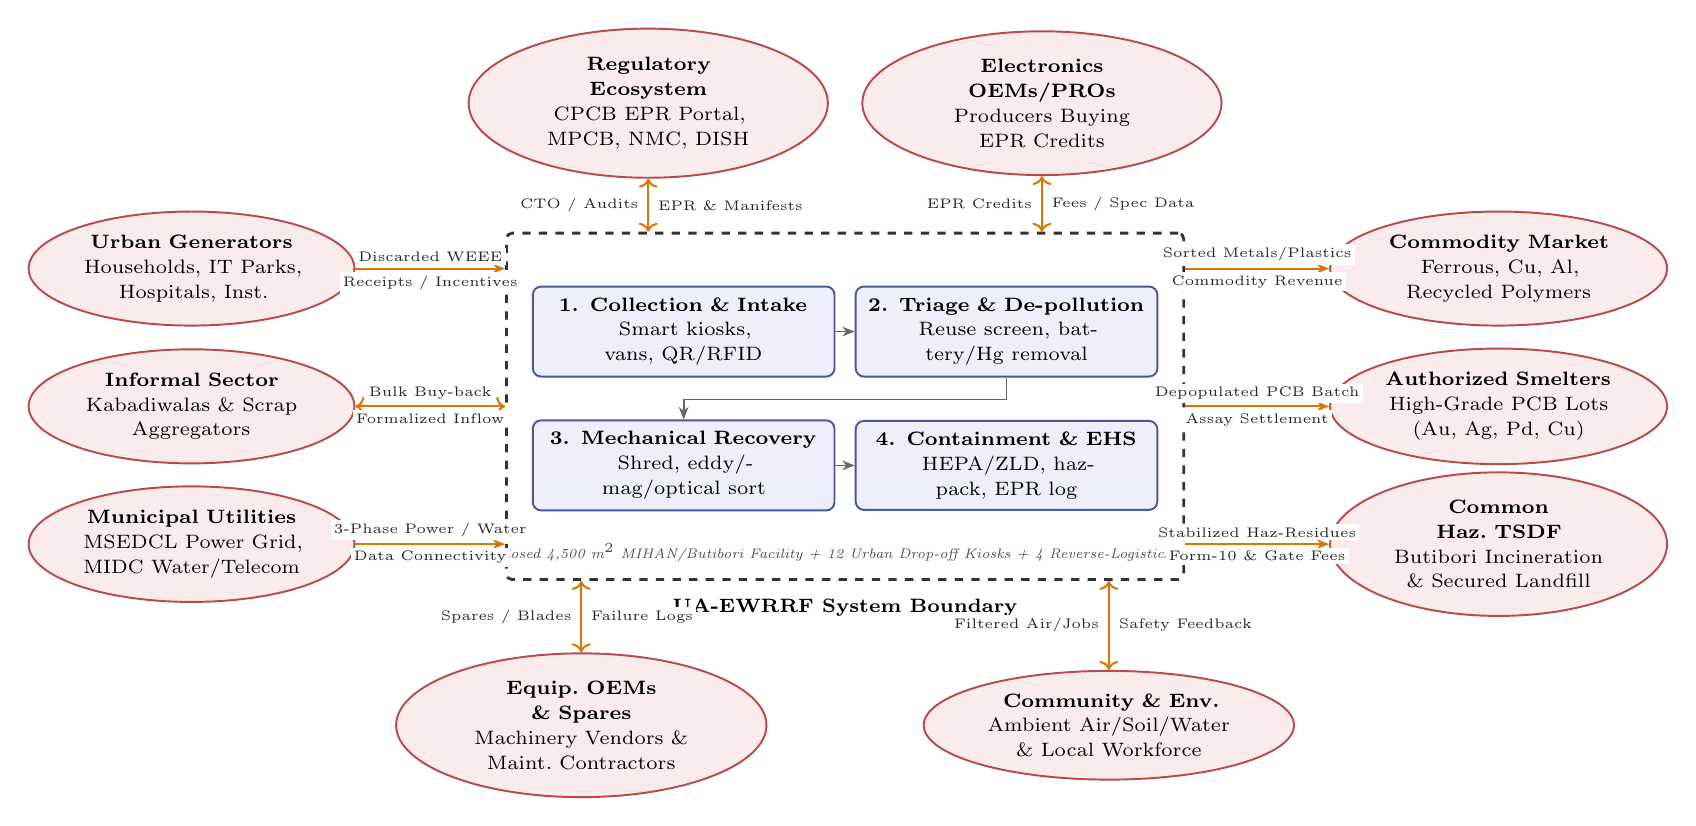
\begin{tikzpicture}[node distance=1.0cm]

% --- Central Dashed System Boundary (exact edit.pdf aesthetic) ---
\node[rectangle, rounded corners=2pt, draw=black!80, dashed, line width=1.0pt, fill=white,
      minimum width=8.6cm, minimum height=4.4cm] (soi) at (0,0) {};

% Internal sub-blocks inside SoI (soft periwinkle-blue rounded boxes)
\node[sebox, text width=3.55cm, minimum height=0.95cm] (s1) at (-2.05, 0.95)
    {\textbf{1. Collection \& Intake}\\Smart kiosks, vans, QR/RFID};
\node[sebox, text width=3.55cm, minimum height=0.95cm] (s2) at (2.05, 0.95)
    {\textbf{2. Triage \& De-pollution}\\Reuse screen, battery/Hg removal};
\node[sebox, text width=3.55cm, minimum height=0.95cm] (s3) at (-2.05, -0.75)
    {\textbf{3. Mechanical Recovery}\\Shred, eddy/mag/optical sort};
\node[sebox, text width=3.55cm, minimum height=0.95cm] (s4) at (2.05, -0.75)
    {\textbf{4. Containment \& EHS}\\HEPA/ZLD, haz-pack, EPR log};

\draw[searrow] (s1.east) -- (s2.west);
\draw[searrow] (s2.south) -- ++(0,-0.28) -| (s3.north);
\draw[searrow] (s3.east) -- (s4.west);

\node[font=\rmfamily\tiny\itshape\color{black!70}, anchor=south] at ($(soi.south)+(0,0.12)$)
    {Enclosed 4,500 m$^2$ MIHAN/Butibori Facility + 12 Urban Drop-off Kiosks + 4 Reverse-Logistics Vans};

% Bold Boundary Caption underneath (matching edit.pdf, centered cleanly between bottom arrows)
\node[font=\rmfamily\scriptsize\bfseries\color{black}, anchor=north] at ($(soi.south)+(0,-0.10)$)
    {UA-EWRRF System Boundary};

% --- External Systems: Soft Rose Ellipses (matching edit.pdf Pages 5 & 12) ---
\node[seboxExt, text width=2.75cm] (ext_gen) at (-8.3, 1.75)
    {\textbf{Urban Generators}\\Households, IT Parks,\\Hospitals, Inst.};

\node[seboxExt, text width=2.75cm] (ext_inf) at (-8.3, 0.0)
    {\textbf{Informal Sector}\\Kabadiwalas \& Scrap\\Aggregators};

\node[seboxExt, text width=2.75cm] (ext_util) at (-8.3, -1.75)
    {\textbf{Municipal Utilities}\\MSEDCL Power Grid,\\MIDC Water/Telecom};

\node[seboxExt, text width=3.05cm] (ext_reg) at (-2.5, 3.85)
    {\textbf{Regulatory Ecosystem}\\CPCB EPR Portal,\\MPCB, NMC, DISH};

\node[seboxExt, text width=3.05cm] (ext_oem) at (2.5, 3.85)
    {\textbf{Electronics OEMs/PROs}\\Producers Buying\\EPR Credits};

\node[seboxExt, text width=2.85cm] (ext_mkt) at (8.3, 1.75)
    {\textbf{Commodity Market}\\Ferrous, Cu, Al,\\Recycled Polymers};

\node[seboxExt, text width=2.85cm] (ext_smelt) at (8.3, 0.0)
    {\textbf{Authorized Smelters}\\High-Grade PCB Lots\\(Au, Ag, Pd, Cu)};

\node[seboxExt, text width=2.85cm] (ext_tsdf) at (8.3, -1.75)
    {\textbf{Common Haz.\ TSDF}\\Butibori Incineration\\\& Secured Landfill};

\node[seboxExt, text width=3.15cm] (ext_sup) at (-3.35, -4.05)
    {\textbf{Equip.\ OEMs \& Spares}\\Machinery Vendors \&\\Maint.\ Contractors};

\node[seboxExt, text width=3.15cm] (ext_com) at (3.35, -4.05)
    {\textbf{Community \& Env.}\\Ambient Air/Soil/Water\\\& Local Workforce};

% --- Warm Orange Boundary-Crossing Arrows (matching edit.pdf) ---
\draw[seextarrow] (ext_gen.east) -- node[selabel, above, yshift=1pt] {Discarded WEEE} node[selabel, below, yshift=-1pt] {Receipts / Incentives} ($(soi.west)+(0,1.75)$);
\draw[seextarrow, <->] (ext_inf.east) -- node[selabel, above, yshift=1pt] {Bulk Buy-back} node[selabel, below, yshift=-1pt] {Formalized Inflow} (soi.west);
\draw[seextarrow] (ext_util.east) -- node[selabel, above, yshift=1pt] {3-Phase Power / Water} node[selabel, below, yshift=-1pt] {Data Connectivity} ($(soi.west)+(0,-1.75)$);

\draw[seextarrow, <->] (ext_reg.south) -- node[selabel, left, xshift=-2pt] {CTO / Audits} node[selabel, right, xshift=2pt] {EPR \& Manifests} ($(soi.north)+(-2.5,0)$);
\draw[seextarrow, <->] (ext_oem.south) -- node[selabel, left, xshift=-2pt] {EPR Credits} node[selabel, right, xshift=2pt] {Fees / Spec Data} ($(soi.north)+(2.5,0)$);

\draw[seextarrow] ($(soi.east)+(0,1.75)$) -- node[selabel, above, yshift=1pt] {Sorted Metals/Plastics} node[selabel, below, yshift=-1pt] {Commodity Revenue} (ext_mkt.west);
\draw[seextarrow] (soi.east) -- node[selabel, above, yshift=1pt] {Depopulated PCB Batch} node[selabel, below, yshift=-1pt] {Assay Settlement} (ext_smelt.west);
\draw[seextarrow] ($(soi.east)+(0,-1.75)$) -- node[selabel, above, yshift=1pt] {Stabilized Haz-Residues} node[selabel, below, yshift=-1pt] {Form-10 \& Gate Fees} (ext_tsdf.west);

\draw[seextarrow, <->] (ext_sup.north) -- node[selabel, left, xshift=-2pt] {Spares / Blades} node[selabel, right, xshift=2pt] {Failure Logs} ($(soi.south)+(-3.35,0)$);
\draw[seextarrow, <->] (ext_com.north) -- node[selabel, left, xshift=-2pt] {Filtered Air/Jobs} node[selabel, right, xshift=2pt] {Safety Feedback} ($(soi.south)+(3.35,0)$);

\end{tikzpicture}%
}
\caption{Context and System Boundary Diagram for the Urban Automated E-Waste Collection, Dismantling, and Resource Recovery Facility (UA-EWRRF).}
\label{fig:context}
\end{figure}


\subsection{Justification of System Boundary}
\begin{itemize}
    \item \textbf{Included inside the boundary:} Kiosks, collection vans, QR/RFID intake, reuse triage, manual hazardous de-pollution (batteries, mercury lamps, capacitors), modular mechanical recovery, HEPA/carbon filtration, zero-liquid-discharge (ZLD) treatment, and temporary hazardous containment. These are directly engineered by the facility designer and govern purity, safety, and EPR compliance.
    \item \textbf{Kept outside the boundary:} Upstream OEM product design, high-temperature pyrometallurgical smelting (viable only at $>30{,}000$ t/yr), final hazardous incineration/landfilling (mandated to authorized Common TSDFs such as Butibori), municipal landfills, and informal street scrap markets. Keeping these external keeps the SoI tractable while defining strict handover interfaces.
\end{itemize}

% ============================================================================
% Section B: Construct the Life Cycle of the Principal System (Deliverable B)
% ============================================================================
\section{Principal-System Life Cycle}
\label{sec:B}

The UA-EWRRF life cycle spans $\approx 18$ years (2 years acquisition, 15 years operation/upgrading, 1 year retirement). Rather than a rigid one-way sequence, commissioning defects, operational safety logs, wear telemetry, and shifting WEEE composition drive continuous feedback into design and mid-life upgrades (Figure~\ref{fig:principal_lc}). Table~\ref{tab:annexB} summarizes each phase (Annexure~B).

% ============================================================================
% Figure 2: Principal-System Life-Cycle Diagram with Iterations & Feedback
% (Deliverable B — Classic Academic Serif Style)
% ============================================================================
\begin{figure}[htbp]
\centering
\resizebox{\textwidth}{!}{%
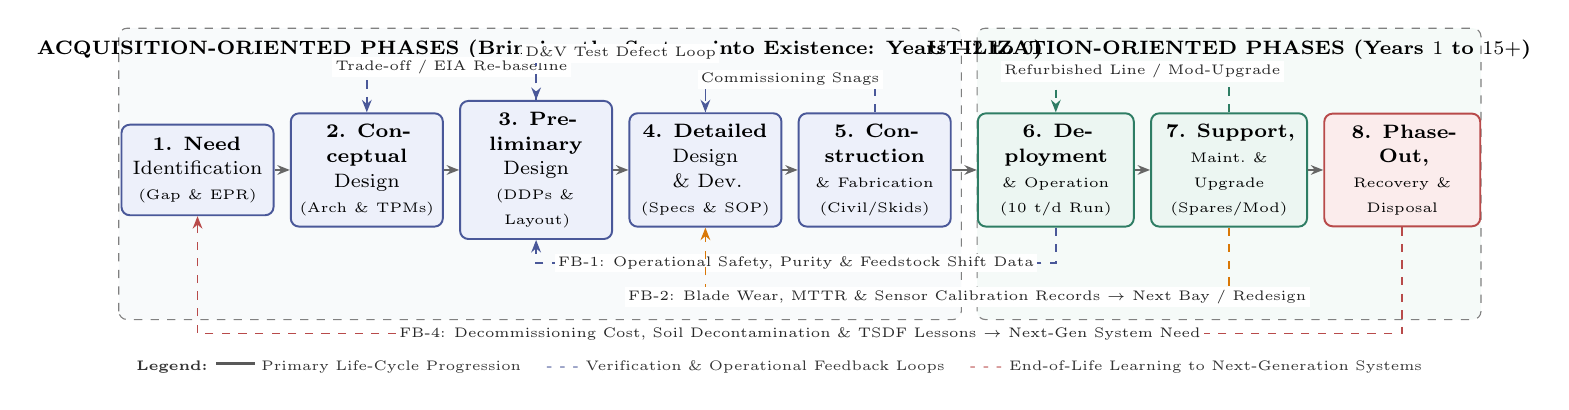
\begin{tikzpicture}[node distance=0.55cm]

% Subtle dashed acquisition vs utilization bands
\draw[dashed, draw=black!50, fill=LightTint!50, rounded corners=3pt] (-0.35, -1.15) rectangle (10.35, 2.55);
\draw[dashed, draw=black!50, fill=DiagTealFill!55, rounded corners=3pt] (10.55, -1.15) rectangle (16.95, 2.55);

\node[font=\rmfamily\scriptsize\bfseries\color{black}] at (5.0, 2.28)
    {ACQUISITION-ORIENTED PHASES (Bringing the System into Existence: Years $-2$ to $0$)};
\node[font=\rmfamily\scriptsize\bfseries\color{black}] at (13.75, 2.28)
    {UTILIZATION-ORIENTED PHASES (Years $1$ to $15+$)};

% 8 Phases
\node[sebox, text width=1.65cm, minimum height=1.15cm] (p1) at (0.65, 0.75) {\textbf{1. Need}\\Identification\\{\tiny(Gap \& EPR)}};
\node[sebox, text width=1.65cm, minimum height=1.15cm] (p2) at (2.80, 0.75) {\textbf{2. Conceptual}\\Design\\{\tiny(Arch \& TPMs)}};
\node[sebox, text width=1.65cm, minimum height=1.15cm] (p3) at (4.95, 0.75) {\textbf{3. Preliminary}\\Design\\{\tiny(DDPs \& Layout)}};
\node[sebox, text width=1.65cm, minimum height=1.15cm] (p4) at (7.10, 0.75) {\textbf{4. Detailed}\\Design \& Dev.\\{\tiny(Specs \& SOP)}};
\node[sebox, text width=1.65cm, minimum height=1.15cm] (p5) at (9.25, 0.75) {\textbf{5. Construction}\\{\tiny\& Fabrication}\\{\tiny(Civil/Skids)}};

\node[seboxTeal, text width=1.70cm, minimum height=1.15cm] (p6) at (11.55, 0.75) {\textbf{6. Deployment}\\{\tiny\& Operation}\\{\tiny(10 t/d Run)}};
\node[seboxTeal, text width=1.70cm, minimum height=1.15cm] (p7) at (13.75, 0.75) {\textbf{7. Support,}\\{\tiny Maint.\ \& Upgrade}\\{\tiny(Spares/Mod)}};
\node[seboxRisk, text width=1.70cm, minimum height=1.15cm] (p8) at (15.95, 0.75) {\textbf{8. Phase-Out,}\\{\tiny Recovery \&}\\{\tiny Disposal}};

% Forward primary arrows
\foreach \i/\j in {p1/p2, p2/p3, p3/p4, p4/p5, p5/p6, p6/p7, p7/p8} {
    \draw[searrow] (\i.east) -- (\j.west);
}

% Short iteration loops (top)
\draw[sefeedback] (p3.north) -- ++(0,0.42) -| node[selabel, pos=0.25] {Trade-off / EIA Re-baseline} (p2.north);
\draw[sefeedback] (p4.north) -- ++(0,0.75) -| node[selabel, pos=0.25] {D\&V Test Defect Loop} (p3.north);
\draw[sefeedback] (p5.north) -- ++(0,0.42) -| node[selabel, pos=0.25] {Commissioning Snags} (p4.north);
\draw[sefeedback, draw=DiagTealDraw] (p7.north) -- ++(0,0.52) -| node[selabel, pos=0.25] {Refurbished Line / Mod-Upgrade} (p6.north);

% Major cross-phase learning feedback loops (bottom)
\draw[sefeedback] (p6.south) -- ++(0,-0.45) -| node[selabel, pos=0.25]
    {FB-1: Operational Safety, Purity \& Feedstock Shift Data} (p3.south);

\draw[sefeedback, draw=DiagOrgDraw] (p7.south) -- ++(0,-0.88) -| node[selabel, pos=0.25]
    {FB-2: Blade Wear, MTTR \& Sensor Calibration Records $\rightarrow$ Next Bay / Redesign} (p4.south);

\draw[seriskarrow] (p8.south) -- ++(0,-1.35) -| node[selabel, pos=0.25]
    {FB-4: Decommissioning Cost, Soil Decontamination \& TSDF Lessons $\rightarrow$ Next-Gen System Need} (p1.south);

% Legend strip
\node[font=\rmfamily\tiny\color{black!80}, anchor=west] at (-0.25, -1.75)
    {\textbf{Legend:} \textcolor{black!65}{\rule[2pt]{14pt}{0.9pt}} Primary Life-Cycle Progression \quad
     \textcolor{DiagBlueDraw}{- - -} Verification \& Operational Feedback Loops \quad
     \textcolor{DiagRedDraw}{- - -} End-of-Life Learning to Next-Generation Systems};

\end{tikzpicture}%
}
\caption{Principal-System Life-Cycle Representation of UA-EWRRF across Eight Phases with Iterations and Feedback Loops.}
\label{fig:principal_lc}
\end{figure}


\begingroup
\footnotesize
\renewcommand{\arraystretch}{1.22}
\begin{xltabular}{\textwidth}{L{2.0cm} Y L{2.35cm} Y L{2.6cm}}
\caption{Principal-system life-cycle analysis for UA-EWRRF (Annexure B format).}
\label{tab:annexB}\\
\toprule
\hdrrow \tblhead{Life-cycle phase} & \tblhead{Principal activities} & \tblhead{Major stakeholders} & \tblhead{Important decisions} & \tblhead{Expected outputs} \\
\midrule
\endfirsthead
\multicolumn{5}{l}{\footnotesize\color{SlateMuted}\textit{Table~\ref{tab:annexB} continued from previous page.}}\\
\toprule
\hdrrow \tblhead{Life-cycle phase} & \tblhead{Principal activities} & \tblhead{Major stakeholders} & \tblhead{Important decisions} & \tblhead{Expected outputs} \\
\midrule
\endhead
\bottomrule
\endfoot

\textbf{1. Need Identification} & Quantify Nagpur WEEE flow, informal leakage, CPCB 2022 EPR quotas, and MIDC plots. & Promoter, NMC, MPCB, OEMs/PROs, Bulk Users. & Target capacity (10 t/d); formal vs.\ aggregator buy-back model. & Needs Statement, Feedstock Study, Site Shortlist. \\
\midrule
\textbf{2. Conceptual Design} & Define boundary, DDPs/DIPs, TPMs, and compare processing architectures. & Promoter, Systems Eng., EHS Cons., Investors. & Select Modular Hybrid (A2); off-site smelting; TPM criteria. & Concept Document, TPM Baseline, EIA Screening. \\
\midrule
\textbf{3. Preliminary Design} & Lay out 4,500 m$^2$ floorplan, negative-pressure bays, HEPA/ZLD, and CTE dossier. & EPC, Process Eng., MPCB, MIDC, OEMs. & Bolted skids vs.\ grouted slabs; bay segregation; EPR API. & PDR Pack, Process Flow Diagrams, MPCB CTE. \\
\midrule
\textbf{4. Detailed Design \& Dev.} & Finalize civil/MEP drawings, blade alloy, optical/XRT specs, fire controls, and SOPs. & EPC, Equip.\ OEMs, Software, DISH, EHS. & Spares depth; quick-swap blades (MTTR $\le 4$ h); Form-10 workflow. & CDR Drawings, BOM, Test Plans, Safety SOPs. \\
\midrule
\textbf{5. Production / Construction} & Lay epoxy containment slab, erect shed, install modular skids \& 12 kiosks, run trials. & EPC, Civil Sub., Equip.\ OEMs, MPCB, Promoter. & QA/QC sign-off; SAT purity ($\ge 95\%$) \& dust ($\le 30$ mg/m$^3$) gates. & Commissioned Plant, Kiosks, Vans, MPCB CTO. \\
\midrule
\textbf{6. Deployment \& Operation} & Daily collection, QR intake, de-pollution, sorting, metal sales, TSDF \& EPR filing. & Ops, EHS, NMC, Generators, Smelters, TSDF. & Daily routing; aggregator pricing; stop-work safety triggers. & Recovered Fractions, PCB Lots, EPR Credits, Manifests. \\
\midrule
\textbf{7. Support, Maint.\ \& Upgrade} & Blade swaps, sensor calibration, HEPA changes, biomonitoring, Year 5--7 retrofits. & Maint.\ Team, OEMs, EHS Lab, Promoter. & Preventive intervals; bay retrofit vs.\ overhaul. & Sustained $A_o \ge 88\%$, Upgraded Bays, Audit Logs. \\
\midrule
\textbf{8. Phase-Out, Recovery \& Disposal} & Halt intake, decontaminate skids/ducts, resell assets, test soil, close CTO. & Decomm.\ Contr., MPCB, MIDC, TSDF, Promoter. & Equipment resale vs.\ scrap; soil remediation scope. & Clean MIDC Plot, Resale Value, MPCB Closure NOC. \\

\end{xltabular}
\endgroup

% ============================================================================
% Section C: Distinguish Acquisition and Utilization (Deliverable C)
% ============================================================================
\section{Acquisition vs.\ Utilization Analysis}
\label{sec:C}

Life-cycle activities divide into two coupled domains:
\begin{itemize}
    \item \textbf{Acquisition-Oriented Activities (Phases 1--5):} Conceiving, permitting (CTE/CTO), building, and commissioning UA-EWRRF. Although CapEx represents only $\approx 25\%$ of total 15-year cost, acquisition decisions lock in over \textbf{70--80\%} of eventual life-cycle cost, safety risk, and maintainability.
    \item \textbf{Utilization-Oriented Activities (Phases 6--8):} Operating collection/recovery lines, maintaining availability, upgrading modules, and retiring the site cleanly. These phases represent over 72\% of total expenditure (power, wages, spares, TSDF gate fees, and closure).
\end{itemize}

Table~\ref{tab:annexC} examines three major acquisition-stage decisions whose impacts surface during utilization.

\begingroup
\footnotesize
\renewcommand{\arraystretch}{1.22}
\begin{xltabular}{\textwidth}{L{2.7cm} L{2.15cm} L{2.65cm} L{2.55cm} Y}
\caption{Acquisition-stage decisions significantly influencing utilization in UA-EWRRF (Annexure C format).}
\label{tab:annexC}\\
\toprule
\hdrrow \tblhead{Acquisition-stage decision} & \tblhead{Decision-maker} & \tblhead{Stakeholders experiencing consequences} & \tblhead{When consequences become visible} & \tblhead{Difficulty of changing later} \\
\midrule
\endfirsthead
\multicolumn{5}{l}{\footnotesize\color{SlateMuted}\textit{Table~\ref{tab:annexC} continued from previous page.}}\\
\toprule
\hdrrow \tblhead{Acquisition-stage decision} & \tblhead{Decision-maker} & \tblhead{Stakeholders experiencing consequences} & \tblhead{When consequences become visible} & \tblhead{Difficulty of changing later} \\
\midrule
\endhead
\bottomrule
\endfoot

\textbf{C1. Shred-first vs.\ pre-depollution hybrid sorting line} & Promoter Board \& EPC (Ph.\ 2--3) & Operators (fire/dust), buyers (impure lots), TSDF (toxic residue). & Years 1--2 via battery fires, alloy contamination, and buyer penalties. & \textbf{Very High:} Requires dismantling primary shredders and halting revenue for 3--5 months. \\
\midrule
\textbf{C2. Proprietary imported machines vs.\ standardized modular skids} & Procurement \& EPC Vendor (Ph.\ 3--4) & Maint.\ team (spare delays), promoter (downtime), OEM EPR clients. & Years 2--7 when imported blades/sensors take 6--10 weeks to replace. & \textbf{High:} Footprints, PLC controls, and power drops are locked to one vendor. \\
\midrule
\textbf{C3. Grouted concrete mounts vs.\ bolted skids on epoxy containment} & Civil EPC \& Cost Controller (Ph.\ 3--5) & Upgrade teams, MPCB, MIDC, decommissioning contractors. & Year 6 upgrades and Year 15 heavy-metal soil excavation audits. & \textbf{Extreme:} Re-pouring slabs beneath heavy machinery requires near-total demolition. \\

\end{xltabular}
\endgroup

\subsection{Stakeholder Alignment Conclusion}
Acquisition and utilization stakeholders are \textbf{only partially aligned}. Both want initial CTO approval and 10 t/day capacity, yet EPC contractors and CapEx-focused sponsors benefit from minimizing construction cost and schedule---favoring grouted mounts or monolithic machinery. Meanwhile, operations, maintenance, EHS staff, and retirement teams absorb the resulting 15-year downtime, dust exposure, retrofit blocks, and remediation liabilities. Resolving this gap requires LCC-based vendor bidding, 3-year OEM availability warranties, and early operator sign-off at PDR/CDR.

% ============================================================================
% Section D: Analyze the Concurrent Life Cycles (Deliverable D)
% ============================================================================
\section{Concurrent Life-Cycle Analysis}
\label{sec:D}

Delivering UA-EWRRF requires managing \textbf{four concurrent life cycles} in parallel from conceptual design onward (Figure~\ref{fig:concurrent_lc}): (1)~the operational recovery plant, (2)~construction and fabrication capability, (3)~support and maintenance infrastructure, and (4)~retirement and site-closure capability. Table~\ref{tab:annexD} summarizes their dependencies and late-development risks (Annexure~D).

% ============================================================================
% Figure 3: Four Concurrent Life Cycles Diagram (Deliverable D)
% ============================================================================
\begin{figure}[htbp]
\centering
\resizebox{\textwidth}{!}{%
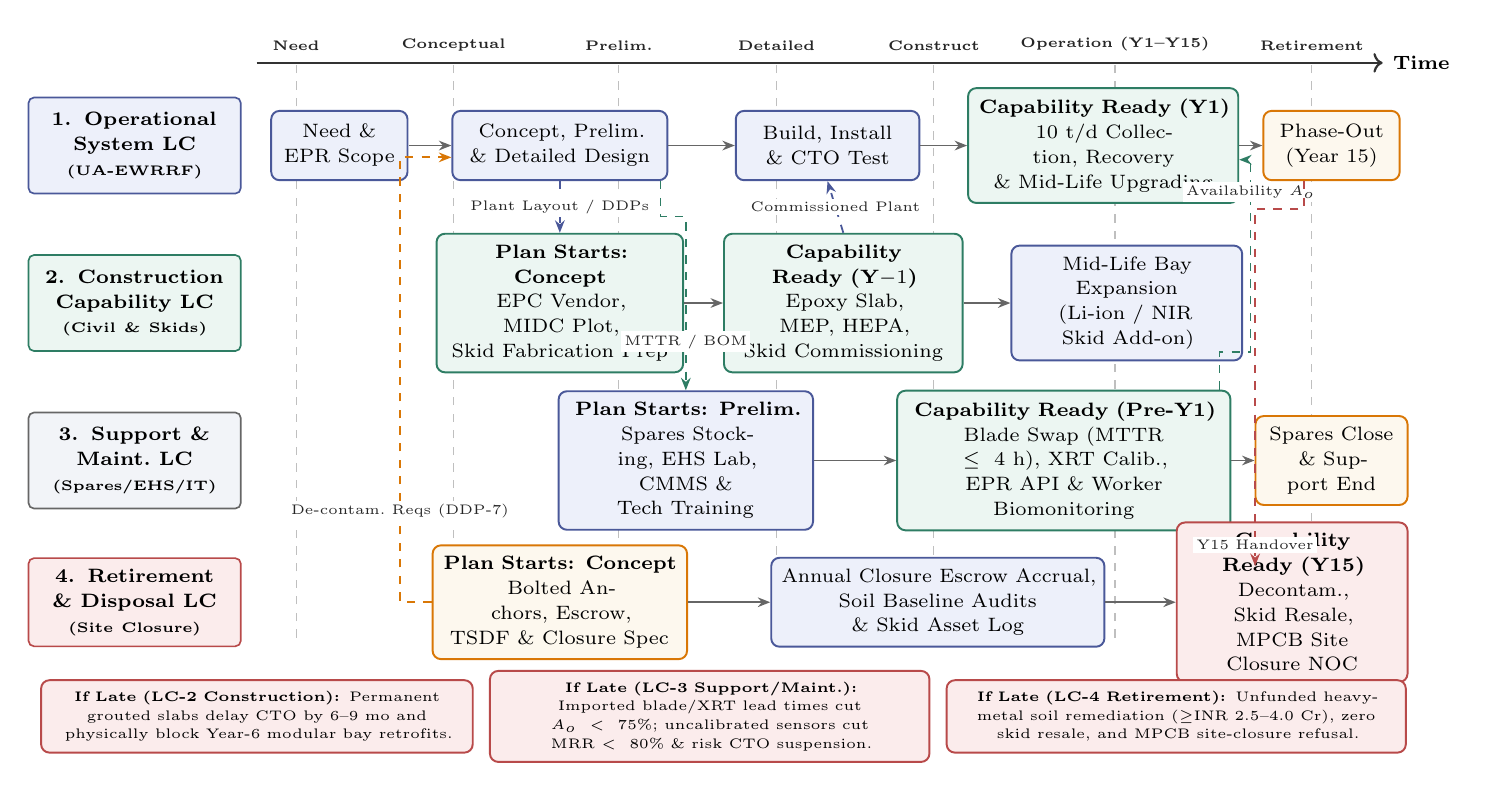
\begin{tikzpicture}

% --- Horizontal Timeline Grid ---
\draw[->, line width=0.8pt, draw=black!80] (2.9, 8.65) -- (17.2, 8.65) node[right, font=\rmfamily\scriptsize\bfseries] {Time};
\foreach \x/\lbl in {3.4/Need, 5.4/Conceptual, 7.5/Prelim., 9.5/Detailed, 11.5/Construct, 13.8/Operation (Y1--Y15), 16.3/Retirement} {
    \draw[dashed, draw=RuleGray] (\x, 1.35) -- (\x, 8.65);
    \node[font=\rmfamily\tiny\bfseries\color{black!85}, above] at (\x, 8.68) {\lbl};
}

% --- Swimlane 1: Product / Operational System Life Cycle (y = 7.6) ---
\node[sebanner, fill=DiagBlueFill, draw=DiagBlueDraw, text width=2.45cm, minimum height=1.22cm]
    (l1) at (1.35, 7.6) {1. Operational\\System LC\\{\tiny(UA-EWRRF)}};

\node[sebox, text width=1.45cm, minimum height=0.88cm] (p_need) at (3.95, 7.6) {Need \&\\EPR Scope};
\node[sebox, text width=2.45cm, minimum height=0.88cm] (p_des)  at (6.75, 7.6) {Concept, Prelim.\\\& Detailed Design};
\node[sebox, text width=2.05cm, minimum height=0.88cm] (p_bld)  at (10.15, 7.6) {Build, Install\\\& CTO Test};
\node[seboxTeal, text width=3.15cm, minimum height=0.88cm] (p_ops) at (13.65, 7.6) {\textbf{Capability Ready (Y1)}\\10 t/d Collection, Recovery\\\& Mid-Life Upgrading};
\node[seboxAmber, text width=1.45cm, minimum height=0.88cm] (p_ret) at (16.55, 7.6) {Phase-Out\\(Year 15)};

\draw[searrow] (p_need) -- (p_des);
\draw[searrow] (p_des) -- (p_bld);
\draw[searrow] (p_bld) -- (p_ops);
\draw[searrow] (p_ops) -- (p_ret);

% --- Swimlane 2: Production / Construction Capability Life Cycle (y = 5.6) ---
\node[sebanner, fill=DiagTealFill, draw=DiagTealDraw, text width=2.45cm, minimum height=1.22cm]
    (l2) at (1.35, 5.6) {2. Construction\\Capability LC\\{\tiny(Civil \& Skids)}};

\node[seboxTeal, text width=2.85cm, minimum height=0.88cm] (c_plan) at (6.75, 5.6) {\textbf{Plan Starts: Concept}\\EPC Vendor, MIDC Plot,\\Skid Fabrication Prep};
\node[seboxTeal, text width=2.75cm, minimum height=0.88cm] (c_exec) at (10.35, 5.6) {\textbf{Capability Ready (Y$-1$)}\\Epoxy Slab, MEP, HEPA,\\Skid Commissioning};
\node[sebox, text width=2.65cm, minimum height=0.88cm] (c_mod)  at (13.95, 5.6) {Mid-Life Bay Expansion\\(Li-ion / NIR Skid Add-on)};

\draw[searrow] (c_plan) -- (c_exec);
\draw[searrow] (c_exec) -- (c_mod);

% --- Swimlane 3: Support & Maintenance System Life Cycle (y = 3.6) ---
\node[sebanner, fill=LightTint, draw=black!60, text width=2.45cm, minimum height=1.22cm]
    (l3) at (1.35, 3.6) {3. Support \&\\Maint.\ LC\\{\tiny(Spares/EHS/IT)}};

\node[sebox, text width=2.95cm, minimum height=0.88cm] (s_plan) at (8.35, 3.6) {\textbf{Plan Starts: Prelim.}\\Spares Stocking, EHS Lab,\\CMMS \& Tech Training};
\node[seboxTeal, text width=3.95cm, minimum height=0.88cm] (s_ops) at (13.15, 3.6) {\textbf{Capability Ready (Pre-Y1)}\\Blade Swap (MTTR $\le 4$ h), XRT Calib.,\\EPR API \& Worker Biomonitoring};
\node[seboxAmber, text width=1.65cm, minimum height=0.88cm] (s_end) at (16.55, 3.6) {Spares Close\\\& Support End};

\draw[searrow] (s_plan) -- (s_ops);
\draw[searrow] (s_ops) -- (s_end);

% --- Swimlane 4: Retirement, Recovery & Disposal System Life Cycle (y = 1.8) ---
\node[sebanner, fill=DiagRedFill, draw=DiagRedDraw, text width=2.45cm, minimum height=1.12cm]
    (l4) at (1.35, 1.8) {4. Retirement\\\& Disposal LC\\{\tiny(Site Closure)}};

\node[seboxAmber, text width=2.95cm, minimum height=0.88cm] (r_plan) at (6.75, 1.8) {\textbf{Plan Starts: Concept}\\Bolted Anchors, Escrow,\\TSDF \& Closure Spec};
\node[sebox, text width=3.95cm, minimum height=0.88cm] (r_esc)  at (11.55, 1.8) {Annual Closure Escrow Accrual,\\Soil Baseline Audits \& Skid Asset Log};
\node[seboxRisk, text width=2.65cm, minimum height=0.88cm] (r_exec) at (16.05, 1.8) {\textbf{Capability Ready (Y15)}\\Decontam., Skid Resale,\\MPCB Site Closure NOC};

\draw[searrow] (r_plan) -- (r_esc);
\draw[searrow] (r_esc) -- (r_exec);

% --- Clean Cross-Cycle Dependencies & Information Exchange Arrows ---
\draw[sefeedback] (p_des.south) -- node[selabel] {Plant Layout / DDPs} (c_plan.north);
\draw[sefeedback] (c_exec.north) -- node[selabel] {Commissioned Plant} (p_bld.south);
\draw[sefeedback, draw=DiagTealDraw] ($(p_des.south east)+(-0.1,0)$) -- ++(0,-0.45) -| node[selabel, pos=0.86] {MTTR / BOM} (s_plan.north);
\draw[sefeedback, draw=DiagTealDraw] ($(s_ops.north east)+(-0.15,0)$) -- ++(0,0.48) -| (15.52, 6.6) |- node[selabel, pos=0.25] {Availability $A_o$} ($(p_ops.east)+(0,-0.18)$);
\draw[sefeedback, draw=DiagOrgDraw] (r_plan.west) -| node[selabel, pos=0.62] {De-contam.\ Reqs (DDP-7)} (4.72, 6.6) |- ($(p_des.west)+(0,-0.15)$);
\draw[seriskarrow] ($(p_ret.south)+(-0.35,0)$) -- ++(0,-0.35) -| (15.58, 2.75) -- node[selabel, pos=0.45] {Y15 Handover} (15.58, 2.26);

% --- Dedicated Bottom Strip: Consequence of Late Development Callouts ---
\node[seboxRisk, text width=5.2cm, minimum height=0.85cm, font=\rmfamily\tiny, anchor=west] at (0.15, 0.35)
    {\textbf{If Late (LC-2 Construction):} Permanent grouted slabs delay CTO by 6--9 mo and physically block Year-6 modular bay retrofits.};

\node[seboxRisk, text width=5.3cm, minimum height=0.85cm, font=\rmfamily\tiny, anchor=west] at (5.85, 0.35)
    {\textbf{If Late (LC-3 Support/Maint.):} Imported blade/XRT lead times cut $A_o < 75\%$; uncalibrated sensors cut MRR $<80\%$ \& risk CTO suspension.};

\node[seboxRisk, text width=5.55cm, minimum height=0.85cm, font=\rmfamily\tiny, anchor=west] at (11.65, 0.35)
    {\textbf{If Late (LC-4 Retirement):} Unfunded heavy-metal soil remediation ($\ge$INR 2.5--4.0 Cr), zero skid resale, and MPCB site-closure refusal.};

\end{tikzpicture}%
}
\caption{Concurrent Life-Cycle Diagram for UA-EWRRF Showing Planning Initiation, Capability Readiness, Inter-Cycle Dependencies, and Late-Consideration Consequences.}
\label{fig:concurrent_lc}
\end{figure}


\begingroup
\footnotesize
\renewcommand{\arraystretch}{1.22}
\begin{xltabular}{\textwidth}{L{2.3cm} Y L{2.0cm} Y Y}
\caption{Analysis of the four concurrent life cycles of UA-EWRRF (Annexure D format).}
\label{tab:annexD}\\
\toprule
\hdrrow \tblhead{Life cycle} & \tblhead{What must be created or prepared?} & \tblhead{When should planning begin?} & \tblhead{Dependence on other life cycles} & \tblhead{Consequence of late consideration} \\
\midrule
\endfirsthead
\multicolumn{5}{l}{\footnotesize\color{SlateMuted}\textit{Table~\ref{tab:annexD} continued from previous page.}}\\
\toprule
\hdrrow \tblhead{Life cycle} & \tblhead{What must be created or prepared?} & \tblhead{When should planning begin?} & \tblhead{Dependence on other life cycles} & \tblhead{Consequence of late consideration} \\
\midrule
\endhead
\bottomrule
\endfoot

\textbf{1. Operational System LC} & 10 t/d plant, sorting skids, HEPA/ZLD, 12 kiosks, 4 vans, EPR portal. & Phase 1 (Need). & Depends on LC-2 build, LC-3 availability ($A_o \ge 88\%$), and LC-4 closure rules. & Unmet EPR quotas, safety incidents, premature obsolescence. \\
\midrule
\textbf{2. Construction Capability LC} & MIDC plot, epoxy slabs, crane rigging, skid jigs, SAT test rigs. & Phase 2 (Concept). & Uses LC-1 DDPs; embeds LC-3 hoist clearances and LC-4 bolted anchors. & 6--9 mo delay; grouted slabs block Year-6 modular upgrades. \\
\midrule
\textbf{3. Support \& Maint.\ LC} & Wear-blade stock, XRT calibration, CMMS, EHS lab, DISH training. & Phase 3 (Prelim.). & Uses LC-1 BOM/MTTR specs; feeds reliability data back to LC-1. & Spare delays cut $A_o < 75\%$; uncalibrated sensors cut MRR $<80\%$. \\
\midrule
\textbf{4. Retirement \& Disposal LC} & Baseline soil survey, closure escrow, TSDF quota, MPCB NOC plan. & Phase 2 (Concept); survey pre-Ph.\ 5. & Imposes DDP-7 constraints on LC-1/LC-2; uses LC-3 incident logs. & Unfunded soil remediation ($\ge$INR 2.5 Cr) \& MPCB closure denial. \\

\end{xltabular}
\endgroup

\subsection{Why Support, Construction, and Retirement Cannot Be Deferred}
\begin{enumerate}
    \item \textbf{Physical Lock-In:} Overhead hoist access, quick-change blade housings (DDP-3), and sealed epoxy containment with bolted skid rails (DDP-7) must be designed before pouring concrete in Phase~5; retrofitting them at Year~15 is physically impossible.
    \item \textbf{Lead-Time Synchronization:} Eddy-current rotors, XRT lamps, and DISH-certified technicians require 4--9 months of preparation before Day-1 startup.
    \item \textbf{Baseline \& Escrow Continuity:} Without a pre-construction soil baseline and Year-1 closure escrow accrual, the promoter cannot legally separate prior industrial contamination from plant operations at Year~15.
\end{enumerate}

% ============================================================================
% Section E: Map the Life-Cycle Functions (Deliverable E)
% ============================================================================
\section{Life-Cycle Functions Mapping}
\label{sec:E}

Sustaining UA-EWRRF across 15+ years requires nine core life-cycle functions spanning design through final site closure (Figure~\ref{fig:lc_functions}). No function belongs solely to one organization; each requires coordinated inputs across operators, EPC vendors, regulators, municipal agencies, and downstream disposal partners (Table~\ref{tab:annexE}).

% ============================================================================
% Figure 4: Life-Cycle Functions & Multi-Stakeholder Map (Deliverable E)
% ============================================================================
\begin{figure}[htbp]
\centering
\resizebox{\textwidth}{!}{%
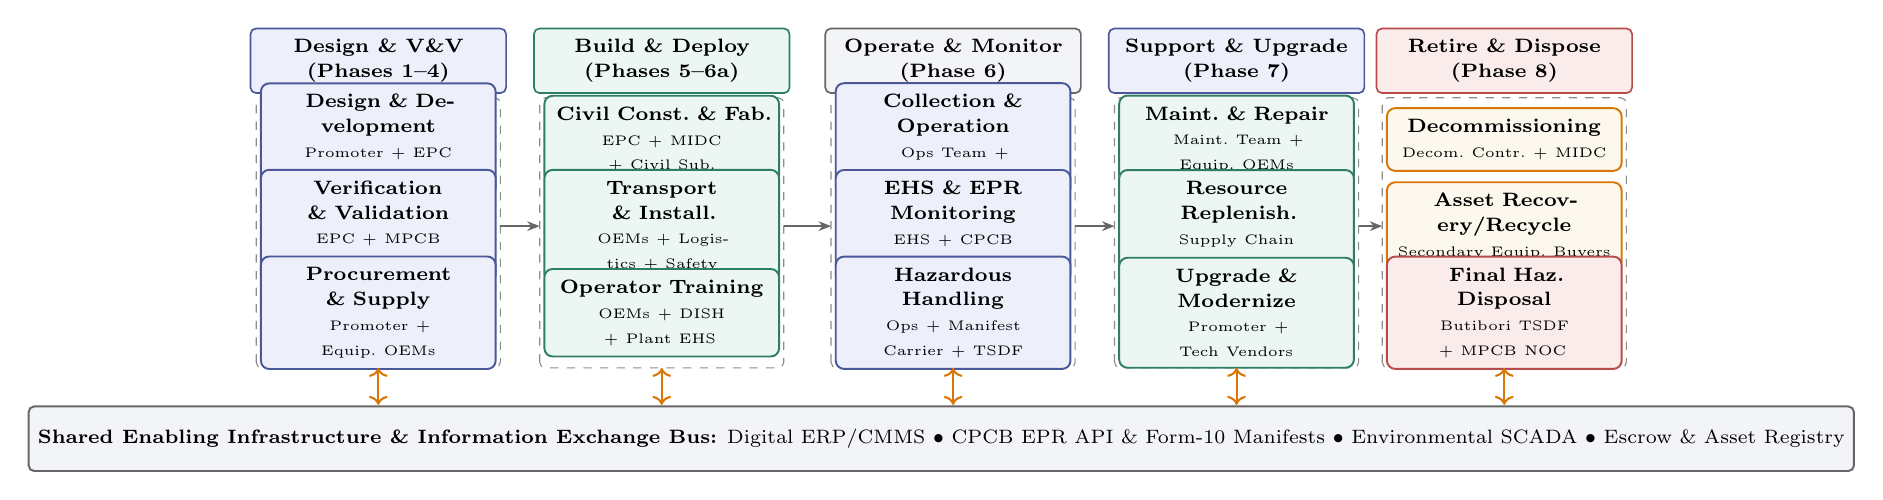
\begin{tikzpicture}

% Column headers (Subtle pastel bordered headers matching edit.pdf)
\foreach \x/\title/\fillcol/\drawcol in {
    1.8/{Design \& V\&V\\(Phases 1--4)}/DiagBlueFill/DiagBlueDraw,
    5.4/{Build \& Deploy\\(Phases 5--6a)}/DiagTealFill/DiagTealDraw,
    9.1/{Operate \& Monitor\\(Phase 6)}/LightTint/black!60,
    12.7/{Support \& Upgrade\\(Phase 7)}/DiagBlueFill/DiagBlueDraw,
    16.1/{Retire \& Dispose\\(Phase 8)}/DiagRedFill/DiagRedDraw%
}{
    \node[sebanner, fill=\fillcol, draw=\drawcol, text width=3.0cm, minimum height=0.82cm]
        at (\x, 5.25) {\title};
    \draw[dashed, draw=black!45, fill=white, rounded corners=2pt] (\x-1.55, 1.35) rectangle (\x+1.55, 4.78);
}

% Functions inside each phase column
\node[sebox, text width=2.7cm] (f1) at (1.8, 4.25) {\textbf{Design \& Development}\\{\tiny Promoter + EPC + EHS Cons.}};
\node[sebox, text width=2.7cm] (f2) at (1.8, 3.15) {\textbf{Verification \& Validation}\\{\tiny EPC + MPCB + 3rd-Party Lab}};
\node[sebox, text width=2.7cm] (f3) at (1.8, 2.05) {\textbf{Procurement \& Supply}\\{\tiny Promoter + Equip.\ OEMs}};

\node[seboxTeal, text width=2.7cm] (f4) at (5.4, 4.25) {\textbf{Civil Const.\ \& Fab.}\\{\tiny EPC + MIDC + Civil Sub.}};
\node[seboxTeal, text width=2.7cm] (f5) at (5.4, 3.15) {\textbf{Transport \& Install.}\\{\tiny OEMs + Logistics + Safety}};
\node[seboxTeal, text width=2.7cm] (f6) at (5.4, 2.05) {\textbf{Operator Training}\\{\tiny OEMs + DISH + Plant EHS}};

\node[sebox, text width=2.7cm] (f7) at (9.1, 4.25) {\textbf{Collection \& Operation}\\{\tiny Ops Team + NMC + Aggreg.}};
\node[sebox, text width=2.7cm] (f8) at (9.1, 3.15) {\textbf{EHS \& EPR Monitoring}\\{\tiny EHS + CPCB Portal + MPCB}};
\node[sebox, text width=2.7cm] (f9) at (9.1, 2.05) {\textbf{Hazardous Handling}\\{\tiny Ops + Manifest Carrier + TSDF}};

\node[seboxTeal, text width=2.7cm] (f10) at (12.7, 4.25) {\textbf{Maint.\ \& Repair}\\{\tiny Maint.\ Team + Equip.\ OEMs}};
\node[seboxTeal, text width=2.7cm] (f11) at (12.7, 3.15) {\textbf{Resource Replenish.}\\{\tiny Supply Chain + MSEDCL}};
\node[seboxTeal, text width=2.7cm] (f12) at (12.7, 2.05) {\textbf{Upgrade \& Modernize}\\{\tiny Promoter + Tech Vendors}};

\node[seboxAmber, text width=2.7cm] (f13) at (16.1, 4.25) {\textbf{Decommissioning}\\{\tiny Decom.\ Contr.\ + MIDC}};
\node[seboxAmber, text width=2.7cm] (f14) at (16.1, 3.15) {\textbf{Asset Recovery/Recycle}\\{\tiny Secondary Equip.\ Buyers}};
\node[seboxRisk, text width=2.7cm] (f15) at (16.1, 2.05) {\textbf{Final Haz.\ Disposal}\\{\tiny Butibori TSDF + MPCB NOC}};

% Cross-cutting Enabling Information & Governance Bus
\node[rectangle, rounded corners=2pt, draw=black!60, fill=LightTint, line width=0.7pt,
      minimum width=17.4cm, minimum height=0.82cm, align=center, font=\rmfamily\scriptsize\color{black}]
    (bus) at (8.95, 0.45)
    {\textbf{Shared Enabling Infrastructure \& Information Exchange Bus:} Digital ERP/CMMS $\bullet$ CPCB EPR API \& Form-10 Manifests $\bullet$ Environmental SCADA $\bullet$ Escrow \& Asset Registry};

% Vertical orange connections to the shared bus
\foreach \x in {1.8, 5.4, 9.1, 12.7, 16.1} {
    \draw[seextarrow, <->] (\x, 1.35) -- (\x, 0.88);
}

% Horizontal flow arrows between stages
\foreach \xa/\xb in {3.35/3.85, 6.95/7.55, 10.65/11.15, 14.25/14.55} {
    \draw[searrow] (\xa, 3.15) -- (\xb, 3.15);
}

\end{tikzpicture}%
}
\caption{Life-Cycle Functions Map for UA-EWRRF Showing Functional Grouping, Multi-Stakeholder Co-Responsibility, and Enabling Systems.}
\label{fig:lc_functions}
\end{figure}


\begingroup
\footnotesize
\renewcommand{\arraystretch}{1.20}
\begin{xltabular}{\textwidth}{L{2.05cm} L{1.35cm} L{2.45cm} L{2.2cm} L{2.1cm} Y}
\caption{Life-cycle functions analysis for UA-EWRRF showing multi-stakeholder co-responsibility (Annexure E format).}
\label{tab:annexE}\\
\toprule
\hdrrow \tblhead{Life-cycle function} & \tblhead{Phase(s)} & \tblhead{Responsible stakeholder(s)} & \tblhead{Enabling resources} & \tblhead{Information exchanged} & \tblhead{Consequence of inadequate performance} \\
\midrule
\endfirsthead
\multicolumn{6}{l}{\footnotesize\color{SlateMuted}\textit{Table~\ref{tab:annexE} continued from previous page.}}\\
\toprule
\hdrrow \tblhead{Life-cycle function} & \tblhead{Phase(s)} & \tblhead{Responsible stakeholder(s)} & \tblhead{Enabling resources} & \tblhead{Information exchanged} & \tblhead{Consequence of inadequate performance} \\
\midrule
\endhead
\bottomrule
\endfoot

\textbf{Design \& Development} & Ph.\ 2--4 & \textit{Primary:} EPC/Sys.\ Eng.; \textit{Contrib.:} Promoter, EHS, OEMs. & CAD/process models, EIA, CPCB manuals. & DDPs, P\&IDs, CTE dossier. & Under-sized filtration, fire hazards, high LCC. \\
\midrule
\textbf{Construction \& Install.} & Ph.\ 5 & \textit{Primary:} EPC \& Civil; \textit{Contrib.:} MIDC, NMC, Equip.\ OEMs. & Epoxy slabs, cranes, kiosks, GPS vans. & As-built drawings, QA/rigging logs. & Leaking slabs, damaged sensors, CTO delay. \\
\midrule
\textbf{Verification \& Validation} & Ph.\ 4--5, 7 & \textit{Primary:} EPC QA \& Lab; \textit{Contrib.:} MPCB, Promoter. & Test WEEE lots, PM monitors, assay lab. & FAT/SAT reports, CTO clearance. & Hidden defects enter service; failed purity gates. \\
\midrule
\textbf{Procurement \& Training} & Ph.\ 4--7 & \textit{Primary:} Supply Chain \& EHS; \textit{Contrib.:} OEMs, DISH, Aggregators. & ERP portal, spare stock, mock bay, PPE. & POs, lead-time alerts, safety certs. & Blade stock-outs; battery puncture fires. \\
\midrule
\textbf{Operation (Collect/Recover)} & Ph.\ 6 & \textit{Primary:} Plant Ops; \textit{Contrib.:} NMC, Bulk Users, Smelters. & Kiosks, vans, de-pollution \& sorting skids. & QR weights, EPR credits, assays. & Low MRR ($<80\%$), impure lots, lost EPR revenue. \\
\midrule
\textbf{EHS \& EPR Monitoring} & Ph.\ 6--8 & \textit{Primary:} EHS Officer; \textit{Contrib.:} CPCB Portal, MPCB, NABL Lab. & PM/VOC sensors, ZLD meters, biomonitoring. & SCADA alerts, Form-10, CPCB API. & Undetected exposure, fines, CTO suspension. \\
\midrule
\textbf{Maint.\ \& Resource Supply} & Ph.\ 6--7 & \textit{Primary:} Maint.\ Team; \textit{Contrib.:} Equip.\ OEMs, MSEDCL, MIDC. & CMMS, gantry hoist, spare blades, grid/solar. & MTBF/MTTR logs, filter pressure. & Chronic downtime ($A_o < 80\%$), missed SLAs. \\
\midrule
\textbf{Upgrading \& Modernization} & Ph.\ 7 & \textit{Primary:} Promoter Eng.; \textit{Contrib.:} Tech Vendors, MPCB. & Reserved modular bay, bolted drops, reserve. & Feedstock mix stats, amended CTO. & Plant becomes obsolete as device chemistry shifts. \\
\midrule
\textbf{Decomm.\ \& Final Disposal} & Ph.\ 8 & \textit{Primary:} Decomm.\ Contr.; \textit{Contrib.:} Butibori TSDF, MPCB, MIDC. & Decontam.\ rigs, soil lab, closure escrow. & Soil assays, Form-10, MPCB NOC. & Toxic legacy, lost resale value, legal penalties. \\

\end{xltabular}
\endgroup

% ============================================================================
% Section F: Translate Life-Cycle Concerns into Design Parameters (F1-F5)
% ============================================================================
\section{Translation of Life-Cycle Concerns into Design Parameters}
\label{sec:F}

Stakeholder concerns are translated systematically into Design Considerations (F1), Design-Dependent Parameters (F2), Design-Independent Parameters (F3), Technical Performance Measures (F4), and Design Criteria (F5).

\subsection{Design Considerations (Annexure F)}
\label{subsec:F1}
Eight system-specific considerations (DC-1 to DC-8) represent acquiring, operating, user, regulatory, environmental, and retirement stakeholders (Table~\ref{tab:annexF}).

\begingroup
\footnotesize
\renewcommand{\arraystretch}{1.20}
\begin{xltabular}{\textwidth}{L{2.7cm} L{2.65cm} L{2.0cm} Y}
\caption{System-specific design considerations for UA-EWRRF (Annexure F format).}
\label{tab:annexF}\\
\toprule
\hdrrow \tblhead{Design consideration} & \tblhead{Stakeholder concerned} & \tblhead{Relevant phase} & \tblhead{Why it should influence the design} \\
\midrule
\endfirsthead
\multicolumn{4}{l}{\footnotesize\color{SlateMuted}\textit{Table~\ref{tab:annexF} continued from previous page.}}\\
\toprule
\hdrrow \tblhead{Design consideration} & \tblhead{Stakeholder concerned} & \tblhead{Relevant phase} & \tblhead{Why it should influence the design} \\
\midrule
\endhead
\bottomrule
\endfoot

\textbf{DC-1. Recovery Yield \& Purity} & Promoter, OEMs, Buyers, Smelters & Ph.\ 2--4, 6 & Drives commodity revenue and CPCB EPR recovery targets; impure streams incur penalties. \\
\midrule
\textbf{DC-2. Throughput \& EPR Traceability} & Promoter, Bulk Users, CPCB, NMC & Ph.\ 2--4, 6 & Clears 10 t/day within CPCB's 180-day storage cap with auditable batch mass balance. \\
\midrule
\textbf{DC-3. Worker Safety \& Fire Control} & Operators, DISH, Community & Ph.\ 2--8 & Punctured Li-ion batteries and lead/mercury dust create severe fire and health hazards. \\
\midrule
\textbf{DC-4. Emission \& ZLD Containment} & MPCB, CPCB, MIDC, Community & Ph.\ 3--8 & Particulate ($\text{PM}_{10}$) or heavy-metal leachate violations trigger immediate CTO revocation. \\
\midrule
\textbf{DC-5. Reliability \& Maintainability} & Maint.\ Team, Operators, Promoter & Ph.\ 3--4, 6--7 & Abrasive PCBs wear shredder blades rapidly; high MTTR breaches pickup SLAs. \\
\midrule
\textbf{DC-6. Modularity \& Adaptability} & Operations, Future Planners, OEMs & Ph.\ 2--3, 7 & Shifting device designs (glued IoT/Li-ion) obsolete rigid monolithic lines early. \\
\midrule
\textbf{DC-7. Energy \& Life-Cycle Affordability} & Promoter, Investors, Society & Ph.\ 1--8 & Balances CapEx, energy OpEx, TSDF fees, and closure cost over 15 years. \\
\midrule
\textbf{DC-8. De-contaminability \& Closure} & Decomm.\ Contr., MPCB, MIDC & Ph.\ 3, 5, 8 & Heavy-metal seepage into unsealed slabs creates multi-crore Year-15 soil liability. \\

\end{xltabular}
\endgroup

\subsection{Design-Dependent Parameters --- DDPs (Annexure G)}
\label{subsec:F2}
Seven DDPs lie directly within UA-EWRRF design authority during conceptual, preliminary, and detailed design (Table~\ref{tab:annexG}).

\begingroup
\footnotesize
\renewcommand{\arraystretch}{1.20}
\begin{xltabular}{\textwidth}{L{2.7cm} Y L{2.45cm} Y}
\caption{Design-Dependent Parameters (DDPs) under UA-EWRRF design authority (Annexure G format).}
\label{tab:annexG}\\
\toprule
\hdrrow \tblhead{DDP} & \tblhead{Design decision influencing it} & \tblhead{Stakeholder affected} & \tblhead{Life-cycle consequence} \\
\midrule
\endfirsthead
\multicolumn{4}{l}{\footnotesize\color{SlateMuted}\textit{Table~\ref{tab:annexG} continued from previous page.}}\\
\toprule
\hdrrow \tblhead{DDP} & \tblhead{Design decision influencing it} & \tblhead{Stakeholder affected} & \tblhead{Life-cycle consequence} \\
\midrule
\endhead
\bottomrule
\endfoot

\textbf{DDP-1. Line Modularity} & Skid-mounted bays with quick-connect utilities vs.\ monolithic train. & EPC, Maint., Upgrade Team. & Allows Year-6 Li-ion/NIR add-ons without plant shutdown; aids asset resale. \\
\midrule
\textbf{DDP-2. Sorting Architecture} & Manual de-pollution + granulator + magnetic, eddy \& optical/XRT skids. & Ops, Buyers, Smelters, TSDF. & Governs purity ($\ge 95\%$), MRR ($\ge 82\%$), and prevents shredder battery fires. \\
\midrule
\textbf{DDP-3. Maintainability (MTTR)} & Quick-swap blade cassettes, overhead hoist, dual baghouse fans. & Maint.\ Team, Ops, OEMs. & Sustains $A_o \ge 88\%$ despite PCB wear; removes single-point air-filter failures. \\
\midrule
\textbf{DDP-4. Dust \& ZLD Containment} & Negative-pressure hoods, HEPA/carbon scrubbers, closed ZLD loop. & Ops, MPCB, Community. & Holds stack $\text{PM} \le 30$ and work-zone $\le 2\text{ mg/m}^3$; zero liquid discharge. \\
\midrule
\textbf{DDP-5. Digital EPR Integration} & QR/RFID tags, digital weighbridge, CPCB EPR \& Form-10 API. & EHS, CPCB, OEMs, Users. & Eliminates mass-balance errors and accelerates EPR credit settlement. \\
\midrule
\textbf{DDP-6. Specific Energy Intensity} & VFD motors on shredders/blowers; dry mechanical over wet thermal sorting. & Promoter, MSEDCL, Society. & Holds SEC $\le 180\text{ kWh/t}$, insulating OpEx from electricity tariff hikes. \\
\midrule
\textbf{DDP-7. De-contaminable Floor} & Impermeable epoxy secondary containment slab + bolted skid anchors. & Civil EPC, MPCB, MIDC, Decomm. & Blocks heavy-metal soil seepage; cuts Year-15 closure cost by $>60\%$. \\

\end{xltabular}
\endgroup

\subsection{Design-Independent Parameters --- DIPs (Annexure H)}
\label{subsec:F3}
Five DIPs are external regulatory, market, and utility forces strictly outside the facility's design boundary and authority (Table~\ref{tab:annexH}).

\begingroup
\footnotesize
\renewcommand{\arraystretch}{1.20}
\begin{xltabular}{\textwidth}{L{2.5cm} L{2.25cm} L{2.2cm} L{2.25cm} Y}
\caption{Design-Independent Parameters (DIPs) external to UA-EWRRF design authority (Annexure H format).}
\label{tab:annexH}\\
\toprule
\hdrrow \tblhead{DIP} & \tblhead{External source} & \tblhead{Expected range} & \tblhead{Decision affected} & \tblhead{Effect of uncertainty} \\
\midrule
\endfirsthead
\multicolumn{5}{l}{\footnotesize\color{SlateMuted}\textit{Table~\ref{tab:annexH} continued from previous page.}}\\
\toprule
\hdrrow \tblhead{DIP} & \tblhead{External source} & \tblhead{Expected range} & \tblhead{Decision affected} & \tblhead{Effect of uncertainty} \\
\midrule
\endhead
\bottomrule
\endfoot

\textbf{DIP-1. EPR \& Emission Rules} & MoEFCC / CPCB \& MPCB CTO norms. & 70--80\% EPR; stack PM $\le 30\text{ mg/m}^3$. & Containment (DDP-4), PCB/BFR (D2). & Tighter BFR/Li-ion rules break rigid non-modular lines. \\
\midrule
\textbf{DIP-2. WEEE Volume \& Mix} & Consumer trends, OEM gluing, informal sector. & 8--12 t/d; rising Li-ion, falling CRT. & Throughput sizing, automation mix (D1). & Low inflow raises $\text{LCC}_t$; glued batteries slow triage. \\
\midrule
\textbf{DIP-3. Commodity Prices} & Global LME/MCX metal \& polymer markets. & Cu INR 720--850/kg; Au/Pd $\pm 25\%$. & Sorting purity (DDP-2) \& reserve. & Price drops squeeze margins of high-OpEx plants. \\
\midrule
\textbf{DIP-4. Grid Power Tariff} & MSEDCL / MERC regulated tariffs. & INR 9.0--11.5/kWh (+4--6\%/yr). & VFD selection (DDP-6) \& solar PV. & Tariff spikes severely penalize shred-first plants (A3). \\
\midrule
\textbf{DIP-5. TSDF Fees \& EHS Wages} & Butibori TSDF \& regional labor market. & TSDF INR 12--18k/t; wages +7--10\%/yr. & Pre-sorting depth (D1) \& haz-scope (D2). & High TSDF fees punish impure streams; wages hit A1. \\

\end{xltabular}
\endgroup

\subsection{Technical Performance Measures --- TPMs (Annexure I)}
\label{subsec:F4}
Six measurable TPMs enable quantitative evaluation from conceptual design through operation (Table~\ref{tab:annexI}).

\begingroup
\footnotesize
\renewcommand{\arraystretch}{1.20}
\begin{xltabular}{\textwidth}{L{2.5cm} L{2.25cm} L{2.7cm} L{2.0cm} Y}
\caption{Technical Performance Measures (TPMs) for UA-EWRRF (Annexure I format).}
\label{tab:annexI}\\
\toprule
\hdrrow \tblhead{TPM} & \tblhead{Related DDPs \& DIPs} & \tblhead{Unit / assessment method} & \tblhead{Phase assessed} & \tblhead{Responsible stakeholder} \\
\midrule
\endfirsthead
\multicolumn{5}{l}{\footnotesize\color{SlateMuted}\textit{Table~\ref{tab:annexI} continued from previous page.}}\\
\toprule
\hdrrow \tblhead{TPM} & \tblhead{Related DDPs \& DIPs} & \tblhead{Unit / assessment method} & \tblhead{Phase assessed} & \tblhead{Responsible stakeholder} \\
\midrule
\endhead
\bottomrule
\endfoot

\textbf{TPM-1. Material Recovery Rate (MRR)} & DDP-1,2,5; DIP-1,2 & \% intake mass recovered at $\ge 95\%$ metal purity; weighbridge \& assay. & Ph.\ 2--4, 5 (SAT), 6. & Plant Ops, Quality Lab \& CPCB Auditor. \\
\midrule
\textbf{TPM-2. Availability ($A_o$)} & DDP-1,3; DIP-2,5 & \% of 2,400 h/yr operational: $\text{MTBF}/(\text{MTBF}+\text{MTTR})$ via CMMS. & Ph.\ 3--4, 6--7. & Maintenance Mgr \& Equip.\ OEM. \\
\midrule
\textbf{TPM-3. Throughput ($Q_p$)} & DDP-1,2,3; DIP-2 & Metric tonnes/day (t/d) at compliant purity \& safety; SCADA count. & Ph.\ 2--3, 5, 6. & Plant Ops Mgr \& EPC (SAT). \\
\midrule
\textbf{TPM-4. Emission \& ZLD ($E_{\text{PM}}$)} & DDP-4,7; DIP-1 & Stack/work-zone $\text{PM}_{10}$ ($\text{mg/m}^3$) via NABL sampler; \% ZLD reuse. & Ph.\ 4, 5 (CTO), 6--8. & EHS Officer, NABL Lab \& MPCB. \\
\midrule
\textbf{TPM-5. Specific Energy (SEC)} & DDP-2,6; DIP-2,4 & kWh/tonne processed; sub-meter readings / weighbridge mass. & Ph.\ 3--4, 5, 6. & Electrical Eng.\ \& Energy Auditor. \\
\midrule
\textbf{TPM-6. Life-Cycle Cost ($\text{LCC}_t$)} & DDP-1--7; DIP-2--5 & INR/tonne over 15 yr (CapEx + OpEx + maint.\ + TSDF + escrow). & Ph.\ 2--3, 6--8. & Promoter CFO, Sys.\ Eng.\ \& Lenders. \\

\end{xltabular}
\endgroup

\subsection{Design Criteria and Integrated Framework (Annexure J)}
\label{subsec:F5}
Table~\ref{tab:annexJ} defines verifiable target ranges and bases (explicitly noting engineering assumptions), while Figure~\ref{fig:integrated_framework} maps how UA-EWRRF stakeholder concerns flow into design trade-offs and closed-loop feedback.

\begingroup
\footnotesize
\renewcommand{\arraystretch}{1.20}
\begin{xltabular}{\textwidth}{L{2.05cm} L{2.4cm} L{2.55cm} L{2.1cm} Y}
\caption{Design criteria established for UA-EWRRF TPMs (Annexure J format).}
\label{tab:annexJ}\\
\toprule
\hdrrow \tblhead{TPM} & \tblhead{Target / acceptable range} & \tblhead{Basis for criterion} & \tblhead{Stakeholder} & \tblhead{Consequence of non-achievement} \\
\midrule
\endfirsthead
\multicolumn{5}{l}{\footnotesize\color{SlateMuted}\textit{Table~\ref{tab:annexJ} continued from previous page.}}\\
\toprule
\hdrrow \tblhead{TPM} & \tblhead{Target / acceptable range} & \tblhead{Basis for criterion} & \tblhead{Stakeholder} & \tblhead{Consequence of non-achievement} \\
\midrule
\endhead
\bottomrule
\endfoot

\textbf{TPM-1 (MRR)} & $\ge 82\%$ (Target: 85\%; min.\ 80\%) & CPCB EPR targets + WEEE benchmarks (\textit{assumption}). & CPCB, OEMs, Promoter. & EPR shortfall, lost metal revenue, higher TSDF waste. \\
\midrule
\textbf{TPM-2 ($A_o$)} & $\ge 88\%$ (Target: 90\%; MTTR $\le 4$ h) & Need to clear 3,000 t/yr in 300 d (\textit{assumption}). & Promoter, Users, Maint. & Storage exceeds 180-day cap; SLA penalties. \\
\midrule
\textbf{TPM-3 ($Q_p$)} & $\ge 10.0\text{ t/d}$ (Range: 9.5--12.5) & Nagpur catchment forecast (\textit{assumption}). & Promoter, NMC, Users. & Unabsorbed e-waste leaks back to informal sector. \\
\midrule
\textbf{TPM-4 ($E_{\text{PM}}$)} & Stack $\le 30$; Indoor $\le 2.0\text{ mg/m}^3$; ZLD 100\% & MPCB CTO, Air Act \& Factories Act (\textit{regulation}). & MPCB, DISH, Ops, Public. & Stop-work order, CTO suspension, health claims. \\
\midrule
\textbf{TPM-5 (SEC)} & $\le 180\text{ kWh/t}$ (Target: $\le 160$) & Medium dry WEEE plant benchmark (\textit{assumption}). & Promoter, Investors. & Rising power OpEx erodes margin \& carbon benefit. \\
\midrule
\textbf{TPM-6 ($\text{LCC}_t$)} & $\le \text{INR } 18{,}500/\text{t}$ (Target: $\le 16{,}500$) & Viability vs.\ EPR + metal revenue (\textit{assumption}). & Board, Lenders, OEMs. & Negative NPV; unfunded upgrades \& closure escrow. \\

\end{xltabular}
\endgroup

% ============================================================================
% Figure 5: System-Specific Integrated Design Framework Relationship Diagram
% (Deliverable F4 / End of Section F)
% Non-floating minipage + \captionof ensures exact inline placement after Table 9
% ============================================================================
\noindent\begin{minipage}{\textwidth}
\vspace{6pt}
\centering
\resizebox{\textwidth}{!}{%
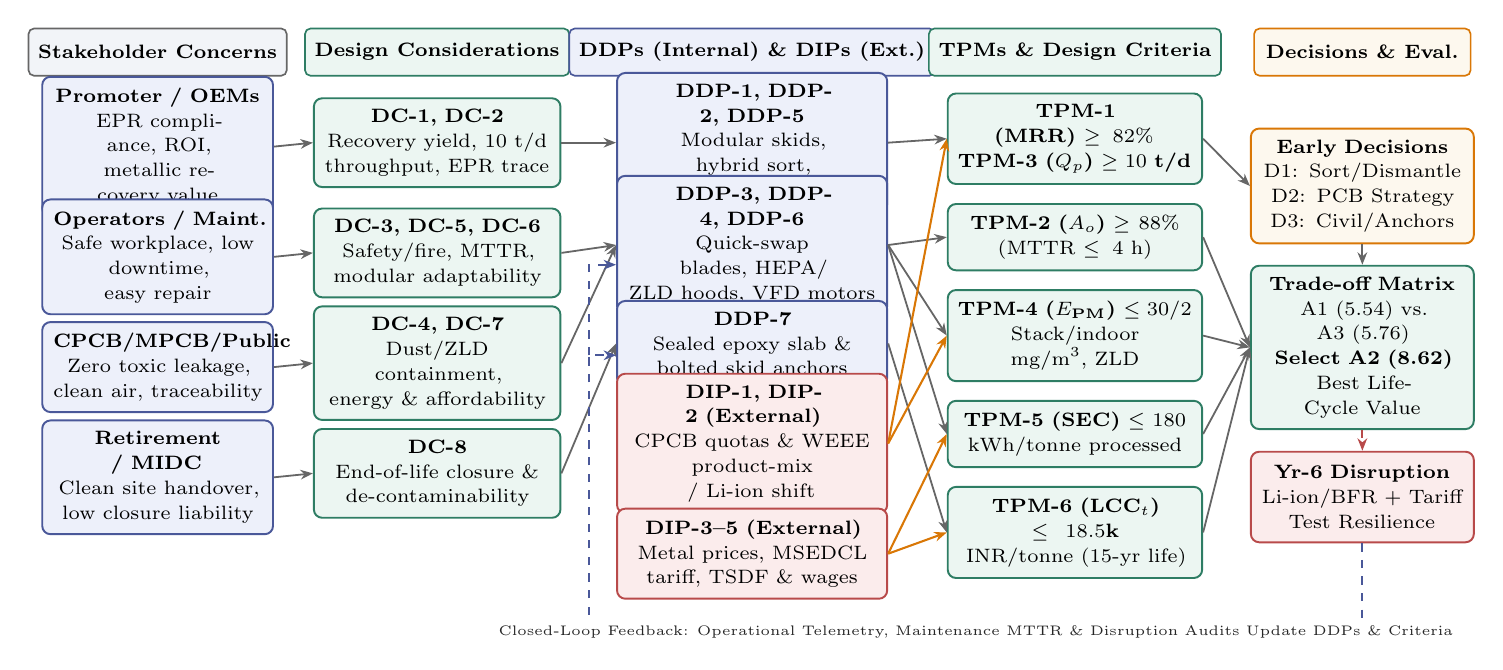
\begin{tikzpicture}[node distance=0.45cm]

% Column Title Banners (clean pastel academic headers)
\node[sebanner, fill=LightTint, draw=black!60, minimum width=2.85cm, minimum height=0.6cm] (h1) at (0, 6.45) {Stakeholder Concerns};
\node[sebanner, fill=DiagTealFill, draw=DiagTealDraw, minimum width=3.05cm, minimum height=0.6cm] (h2) at (3.55, 6.45) {Design Considerations};
\node[sebanner, fill=DiagBlueFill, draw=DiagBlueDraw, minimum width=3.35cm, minimum height=0.6cm] (h3) at (7.55, 6.45) {DDPs (Internal) \& DIPs (Ext.)};
\node[sebanner, fill=DiagTealFill, draw=DiagTealDraw, minimum width=3.15cm, minimum height=0.6cm] (h4) at (11.65, 6.45) {TPMs \& Design Criteria};
\node[sebanner, fill=AmberTint, draw=DiagOrgDraw, minimum width=2.75cm, minimum height=0.6cm] (h5) at (15.30, 6.45) {Decisions \& Eval.};

% --- Col 1: Stakeholder Concerns ---
\node[sebox, text width=2.65cm] (st1) at (0, 5.25) {\textbf{Promoter / OEMs}\\EPR compliance, ROI,\\metallic recovery value};
\node[sebox, text width=2.65cm] (st2) at (0, 3.85) {\textbf{Operators / Maint.}\\Safe workplace, low\\downtime, easy repair};
\node[sebox, text width=2.65cm] (st3) at (0, 2.45) {\textbf{CPCB/MPCB/Public}\\Zero toxic leakage,\\clean air, traceability};
\node[sebox, text width=2.65cm] (st4) at (0, 1.05) {\textbf{Retirement / MIDC}\\Clean site handover,\\low closure liability};

% --- Col 2: Design Considerations ---
\node[seboxTeal, text width=2.85cm] (dc1) at (3.55, 5.30) {\textbf{DC-1, DC-2}\\Recovery yield, 10 t/d\\throughput, EPR trace};
\node[seboxTeal, text width=2.85cm] (dc2) at (3.55, 3.90) {\textbf{DC-3, DC-5, DC-6}\\Safety/fire, MTTR,\\modular adaptability};
\node[seboxTeal, text width=2.85cm] (dc3) at (3.55, 2.50) {\textbf{DC-4, DC-7}\\Dust/ZLD containment,\\energy \& affordability};
\node[seboxTeal, text width=2.85cm] (dc4) at (3.55, 1.10) {\textbf{DC-8}\\End-of-life closure \&\\de-contaminability};

% --- Col 3: DDPs (Top) & DIPs (Bottom) ---
\node[sebox, text width=3.15cm] (ddp1) at (7.55, 5.30) {\textbf{DDP-1, DDP-2, DDP-5}\\Modular skids, hybrid sort,\\QR/EPR API logging};
\node[sebox, text width=3.15cm] (ddp2) at (7.55, 4.00) {\textbf{DDP-3, DDP-4, DDP-6}\\Quick-swap blades, HEPA/\\ZLD hoods, VFD motors};
\node[sebox, text width=3.15cm] (ddp3) at (7.55, 2.75) {\textbf{DDP-7}\\Sealed epoxy slab \&\\bolted skid anchors};

\node[seboxRisk, text width=3.15cm] (dip1) at (7.55, 1.48) {\textbf{DIP-1, DIP-2 (External)}\\CPCB quotas \& WEEE\\product-mix / Li-ion shift};
\node[seboxRisk, text width=3.15cm] (dip2) at (7.55, 0.08) {\textbf{DIP-3--5 (External)}\\Metal prices, MSEDCL\\tariff, TSDF \& wages};

% --- Col 4: TPMs & Criteria ---
\node[seboxTeal, text width=2.95cm] (tpm1) at (11.65, 5.35) {\textbf{TPM-1 (MRR) $\ge 82\%$}\\\textbf{TPM-3 ($Q_p$) $\ge 10$ t/d}};
\node[seboxTeal, text width=2.95cm] (tpm2) at (11.65, 4.10) {\textbf{TPM-2 ($A_o$) $\ge 88\%$}\\(MTTR $\le 4$ h)};
\node[seboxTeal, text width=2.95cm] (tpm3) at (11.65, 2.85) {\textbf{TPM-4 ($E_{\text{PM}}$) $\le 30/2$}\\Stack/indoor mg/m$^3$, ZLD};
\node[seboxTeal, text width=2.95cm] (tpm4) at (11.65, 1.60) {\textbf{TPM-5 (SEC) $\le 180$}\\kWh/tonne processed};
\node[seboxTeal, text width=2.95cm] (tpm5) at (11.65, 0.35) {\textbf{TPM-6 ($\text{LCC}_t$) $\le 18.5$k}\\INR/tonne (15-yr life)};

% --- Col 5: Decisions, Trade-offs & Disruption ---
\node[seboxAmber, text width=2.55cm, minimum height=1.35cm] (ev1) at (15.30, 4.75) {\textbf{Early Decisions}\\D1: Sort/Dismantle\\D2: PCB Strategy\\D3: Civil/Anchors};
\node[seboxTeal, text width=2.55cm, minimum height=1.45cm] (ev2) at (15.30, 2.70) {\textbf{Trade-off Matrix}\\A1 (5.54) vs.\ A3 (5.76)\\\textbf{Select A2 (8.62)}\\Best Life-Cycle Value};
\node[seboxRisk, text width=2.55cm, minimum height=1.15cm] (ev3) at (15.30, 0.80) {\textbf{Yr-6 Disruption}\\Li-ion/BFR + Tariff\\Test Resilience};

% Connecting Arrows
\draw[searrow] (st1.east) -- (dc1.west);
\draw[searrow] (st2.east) -- (dc2.west);
\draw[searrow] (st3.east) -- (dc3.west);
\draw[searrow] (st4.east) -- (dc4.west);

\draw[searrow] (dc1.east) -- (ddp1.west);
\draw[searrow] (dc2.east) -- (ddp2.west);
\draw[searrow] (dc3.east) -- (ddp2.west);
\draw[searrow] (dc4.east) -- (ddp3.west);

\draw[searrow] (ddp1.east) -- (tpm1.west);
\draw[searrow] (ddp2.east) -- (tpm2.west);
\draw[searrow] (ddp2.east) -- (tpm3.west);
\draw[searrow] (ddp2.east) -- (tpm4.west);
\draw[searrow] (ddp3.east) -- (tpm5.west);

\draw[seextarrow] (dip1.east) -- (tpm1.west);
\draw[seextarrow] (dip1.east) -- (tpm3.west);
\draw[seextarrow] (dip2.east) -- (tpm4.west);
\draw[seextarrow] (dip2.east) -- (tpm5.west);

\draw[searrow] (tpm1.east) -- (ev1.west);
\draw[searrow] (tpm2.east) -- (ev2.west);
\draw[searrow] (tpm3.east) -- (ev2.west);
\draw[searrow] (tpm4.east) -- (ev2.west);
\draw[searrow] (tpm5.east) -- (ev2.west);
\draw[searrow] (ev1.south) -- (ev2.north);
\draw[seriskarrow] (ev2.south) -- (ev3.north);

% Clean orthogonal closed-loop feedback routed underneath DIP boxes and up open channel x=5.48
\draw[sefeedback]
    (ev3.south) -- (15.30, -0.92)
    -- node[selabel] {Closed-Loop Feedback: Operational Telemetry, Maintenance MTTR \& Disruption Audits Update DDPs \& Criteria}
    (5.48, -0.92) |- ($(ddp3.west)+(0,-0.15)$);
\draw[sefeedback] (5.48, 2.60) |- ($(ddp2.west)+(0,-0.25)$);

\end{tikzpicture}%
}
\captionof{figure}{System-Specific Integrated Design Framework for UA-EWRRF Tracing Stakeholder Concerns through Design Considerations, DDPs, DIPs, TPMs, and Criteria.}
\label{fig:integrated_framework}
\vspace{4pt}
\end{minipage}


% ============================================================================
% Section G: Analyze Early Design Decisions and Their Life-Cycle Consequences
% (Deliverable G)
% ============================================================================
\section{Early Design Decisions and Life-Cycle Consequences}
\label{sec:G}

Three early conceptual/preliminary design decisions govern production/construction (D1, D3), operation/support (D1, D2), and retirement/disposal (D2, D3), summarized in Annexure~K (Table~\ref{tab:annexK}).

\begingroup
\footnotesize
\renewcommand{\arraystretch}{1.20}
\begin{xltabular}{\textwidth}{L{2.4cm} L{1.7cm} L{1.7cm} L{1.7cm} L{1.8cm} Y}
\caption{Early design decisions and traced life-cycle consequences (Annexure K format).}
\label{tab:annexK}\\
\toprule
\hdrrow \tblhead{Early design decision} & \tblhead{Consid.} & \tblhead{DDPs} & \tblhead{DIPs} & \tblhead{TPMs} & \tblhead{Consequences across life cycle} \\
\midrule
\endfirsthead
\multicolumn{6}{l}{\footnotesize\color{SlateMuted}\textit{Table~\ref{tab:annexK} continued from previous page.}}\\
\toprule
\hdrrow \tblhead{Early design decision} & \tblhead{Consid.} & \tblhead{DDPs} & \tblhead{DIPs} & \tblhead{TPMs} & \tblhead{Consequences across life cycle} \\
\midrule
\endhead
\bottomrule
\endfoot

\textbf{D1. Dismantling \& Sorting Architecture} (Manual vs.\ Hybrid vs.\ Shred-First) & DC-1,2, 3,5,7 & DDP-1, 2,3,6 & DIP-2, 4,5 & TPM-1--6 & Sets CapEx, fire risk, purity, MTTR, power draw, and adaptability to glued/Li-ion devices. \\
\midrule
\textbf{D2. PCB Precious-Metal Strategy} (Dry Pre-Conc.\ + Off-Site Smelter vs.\ Acid Leach) & DC-1,3, 4,7,8 & DDP-2, 4,7 & DIP-1, 3,5 & TPM-1, 4,6 & Dry pre-concentration trades $\approx 5\text{--}8\%$ local Au/Pd margin to avoid heavy acid ETP CapEx, corrosion, and toxic sludge. \\
\midrule
\textbf{D3. Civil Containment \& Foundations} (Bolted Skids on Epoxy vs.\ Grouted Concrete) & DC-4,6, 7,8 & DDP-1, 7 & DIP-1, 2,5 & TPM-4, 6 & Adds $\approx\text{INR } 55$ lakh civil CapEx (+7\%) but enables Year-6 retrofits and saves $>$INR 2.2 Cr in Year-15 soil cleanup. \\

\end{xltabular}
\endgroup

\subsection{Life-Cycle Consequence Analysis}

\subsubsection*{Decision D1: Dismantling \& Sorting Architecture (Acquisition--Utilization Paradox)}
\begin{enumerate}
    \item \textbf{Immediate Benefit:} A monolithic shred-first line promises 15 t/day headline throughput with minimal headcount, while a manual shop minimizes initial CapEx (INR 3.2 Cr).
    \item \textbf{Production/Construction:} Shred-first needs heavy concrete foundations, 630 kVA transformers, and long import lead times; modular hybrid skids use standard drops and commission faster.
    \item \textbf{Operation \& Support (Paradox):} Shred-first detonates unremoved Li-ion cells, causing fires, cross-contaminated streams (MRR 79\%), high power draw (245 kWh/t), and 14-h jam repairs ($A_o = 78\%$). Manual lines breach indoor dust limits ($2.6\text{ mg/m}^3$). Hybrid de-pollution + optical/eddy skids balance safety and purity.
    \item \textbf{Upgrading:} Monolithic lines halt completely during retrofits; modular skids accept bay-by-bay NIR/Li-ion upgrades.
    \item \textbf{Retirement/Sustainability:} Shred-first increases hazardous TSDF fines by 35--45\% and complicates Year-15 duct decontamination.
    \item \textbf{Difficulty to Change Later:} \textbf{Very High} --- requires tearing out conveyors and halting revenue for 3--5 months.
\end{enumerate}

\subsubsection*{Decision D2: PCB Precious-Metal \& Hazardous Fraction Strategy}
\begin{enumerate}
    \item \textbf{Immediate Benefit:} On-site acid hydrometallurgy appears to retain local Au/Pd refining margins instead of paying external smelter fees.
    \item \textbf{Production/Construction:} Acid leaching adds +INR 4.5 Cr CapEx, acid-proof tanks, wet scrubbers, and 9--12 months of stricter EIA/CTE permitting; dry pre-concentration builds cleanly and fast.
    \item \textbf{Operation \& Support:} Wet leaching brings pump corrosion, scarce chemical staff (DIP-5), acid fume hazards, and toxic sludge; dry mechanical concentration uses standard mechanical support.
    \item \textbf{Upgrading:} Chemical plants are regulatory-locked; dry lines easily swap electrostatic/eddy modules.
    \item \textbf{Retirement/Sustainability:} Acid leaching leaves severe drain/tank contamination at Year~15; dry pre-concentration keeps chemical legacy minimal.
    \item \textbf{Difficulty to Change Later:} \textbf{High} --- removing an acid plant mid-life is punitive, and adding one requires fresh EIA clearance.
\end{enumerate}

\subsubsection*{Decision D3: Civil Containment \& Modular Foundation Strategy}
\begin{enumerate}
    \item \textbf{Immediate Benefit:} Plain concrete with grouted anchor bolts saves $\approx\text{INR } 55$ lakh during Phase~5 civil works.
    \item \textbf{Production/Construction:} Epoxy secondary containment with bolted rails adds $\approx 3$ weeks curing and bund detailing.
    \item \textbf{Operation \& Support:} Seamless epoxy floors enable rapid HEPA dust cleanup and instant electrolyte-spill detection ($\text{PM} \le 2.0\text{ mg/m}^3$).
    \item \textbf{Upgrading:} Bolted skids swap obsolete units in 10--14 days without breaking concrete.
    \item \textbf{Retirement/Sustainability:} Bolted skids retain 20--30\% resale value and sealed floors prevent soil seepage, avoiding $>$INR 2.2 Cr in excavation remediation.
    \item \textbf{Difficulty to Change Later:} \textbf{Extreme} --- cannot retrofit beneath active heavy machinery without demolition.
\end{enumerate}

% ============================================================================
% Section H: Evaluate Alternative Life-Cycle Designs (Deliverable H)
% ============================================================================
\section{Evaluation of Alternative Life-Cycle Designs}
\label{sec:H}

We evaluate \textbf{Decision D1} across three feasible architectures:
\begin{itemize}
    \item \textbf{Alternative 1 (A1) --- Manual-Intensive + Basic Shredder:} Low CapEx ($\approx\text{INR } 3.2\text{ Cr}$); 45--50 manual workers + coarse shredder and magnetic belt.
    \item \textbf{Alternative 2 (A2) --- Modular Hybrid De-pollution + Sensor-Assisted Sorting:} Moderate CapEx ($\approx\text{INR } 7.8\text{ Cr}$); enclosed negative-pressure manual battery/hazard removal feeding bolted granulator, magnetic, eddy-current, and optical/XRT skids (22--25 staff).
    \item \textbf{Alternative 3 (A3) --- Monolithic Automated Shred-First Line:} High CapEx ($\approx\text{INR } 13.5\text{ Cr}$); heavy twin-stage shredders ingesting mixed devices directly (12--14 staff).
\end{itemize}

\subsection{Comparative Evaluation Matrix (Annexure L)}
Weights sum to $1.00$: \textbf{TPM-1 (0.22)} and \textbf{TPM-4 (0.22)} lead because safety is a non-negotiable license-to-operate gate and MRR drives EPR/revenue; \textbf{TPM-6 (0.18)} captures 15-year viability; \textbf{TPM-2 (0.16)} protects SLAs; \textbf{TPM-3 (0.12)} covers catchment capacity; and \textbf{TPM-5 (0.10)} captures energy exposure. Scores use a 1--10 scale ($10=$ high margin above target, $7\text{--}8=$ cleanly passes, $4\text{--}6=$ marginal/fails) based on WEEE plant benchmarks and engineering assumptions (Table~\ref{tab:annexL}).

\begingroup
\footnotesize
\renewcommand{\arraystretch}{1.20}
\begin{xltabular}{\textwidth}{L{2.35cm} L{2.45cm} Y Y Y}
\caption{Evaluation of three design alternatives for Decision D1 against TPMs and criteria (Annexure L format).}
\label{tab:annexL}\\
\toprule
\hdrrow \tblhead{TPM (Weight)} & \tblhead{Design criterion} & \tblhead{Alternative 1 (Manual)} & \tblhead{Alternative 2 (Modular Hybrid)} & \tblhead{Alternative 3 (Shred-First)} \\
\midrule
\endfirsthead
\multicolumn{5}{l}{\footnotesize\color{SlateMuted}\textit{Table~\ref{tab:annexL} continued from previous page.}}\\
\toprule
\hdrrow \tblhead{TPM (Weight)} & \tblhead{Design criterion} & \tblhead{Alternative 1 (Manual)} & \tblhead{Alternative 2 (Modular Hybrid)} & \tblhead{Alternative 3 (Shred-First)} \\
\midrule
\endhead
\bottomrule
\endfoot

\textbf{TPM-1: MRR} (0.22) & $\ge 82\%$ ($\ge 95\%$ purity) & \textbf{76\%} \textcolor{CrimsonRisk}{(Fail)} --- Poor PCB recovery. \textit{Score: 5} & \textbf{86\%} \textcolor{TealAccent}{(Pass)} --- Clean optical/eddy purity. \textit{Score: 9} & \textbf{79\%} \textcolor{CrimsonRisk}{(Fail)} --- Cross-contamination. \textit{Score: 6} \\
\midrule
\textbf{TPM-2: $A_o$} (0.16) & $\ge 88\%$ (MTTR $\le 4$ h) & \textbf{92\%} \textcolor{TealAccent}{(Pass)} --- Simple tools. \textit{Score: 8} & \textbf{90\%} \textcolor{TealAccent}{(Pass)} --- Parallel bays, MTTR 3.5 h. \textit{Score: 8} & \textbf{78\%} \textcolor{CrimsonRisk}{(Fail)} --- Jams \& fires, MTTR 14 h. \textit{Score: 5} \\
\midrule
\textbf{TPM-3: $Q_p$} (0.12) & $\ge 10.0\text{ t/d}$ & \textbf{6.5 t/d} \textcolor{CrimsonRisk}{(Fail)} --- Labor bottleneck. \textit{Score: 4} & \textbf{11.0 t/d} \textcolor{TealAccent}{(Pass)} --- Scalable 2nd shift. \textit{Score: 8} & \textbf{15.0 t/d} \textcolor{TealAccent}{(Pass)} --- Peak raw speed. \textit{Score: 10} \\
\midrule
\textbf{TPM-4: $E_{\text{PM}}$} (0.22) & $\le 30 / 2.0\text{ mg/m}^3$; ZLD & \textbf{28 / 2.6} \textcolor{CrimsonRisk}{(Fail)} --- Open indoor dust. \textit{Score: 4} & \textbf{16 / 1.1} \textcolor{TealAccent}{(Pass)} --- Enclosed HEPA/ZLD. \textit{Score: 9} & \textbf{24 / 1.9} \textcolor{AmberWarn}{(Marg.)} --- Fire/VOC spikes. \textit{Score: 6} \\
\midrule
\textbf{TPM-5: SEC} (0.10) & $\le 180\text{ kWh/t}$ & \textbf{95 kWh/t} \textcolor{TealAccent}{(Pass)} --- Low power. \textit{Score: 9} & \textbf{155 kWh/t} \textcolor{TealAccent}{(Pass)} --- VFD dry sorting. \textit{Score: 8} & \textbf{245 kWh/t} \textcolor{CrimsonRisk}{(Fail)} --- Twin shredders. \textit{Score: 4} \\
\midrule
\textbf{TPM-6: $\text{LCC}_t$} (0.18) & $\le \text{INR } 18{,}500/\text{t}$ & \textbf{19,200/t} \textcolor{CrimsonRisk}{(Fail)} --- High wage/TSDF. \textit{Score: 5} & \textbf{16,200/t} \textcolor{TealAccent}{(Pass)} --- Best 15-yr LCC. \textit{Score: 9} & \textbf{20,400/t} \textcolor{CrimsonRisk}{(Fail)} --- CapEx/power/sludge. \textit{Score: 4} \\
\midrule
\subhdrrow \textbf{Weighted Total} & \textbf{Criteria Passed} & \textbf{5.54 / 10} (2/6 passed) & \textbf{8.62 / 10} (\textbf{6/6 passed}) & \textbf{5.76 / 10} (2/6 passed) \\

\end{xltabular}
\endgroup

\subsection{Recommendation and Systems Interpretation}
We recommend \textbf{Alternative 2 (Modular Hybrid, 8.62/10)}---not solely for its top score, but because it is the \textbf{only design meeting all six criteria} without offloading risk onto operators or site retirement:
\begin{enumerate}
    \item \textbf{Criteria Satisfied:} Passes all six gates---MRR (86\%), $A_o$ (90\%), $Q_p$ (11.0 t/d), $E_{\text{PM}}$ (16/1.1 $\text{mg/m}^3$), SEC (155 kWh/t), and $\text{LCC}_t$ (INR 16,200/t).
    \item \textbf{Where It Falls Short:} Higher initial CapEx than A1 (+INR 4.6 Cr), lower raw burst speed than A3 (11 vs.\ 15 t/d), and ongoing optical/XRT calibration needs.
    \item \textbf{Stakeholders Benefiting:} Operators and neighbors (clean air, fire safety), OEMs/buyers (high purity, steady EPR credits), and maintenance/closure teams (bolted modular skids).
    \item \textbf{Stakeholders Bearing Extra Cost/Risk:} Promoters carry moderate upfront financing cost, and maintenance must retain sensor-calibration technicians (mitigated via OEM AMC).
    \item \textbf{DIPs That Could Shift the Result:} Severe skilled-labor scarcity (\textbf{DIP-5}) or a mandatory surge to $>25\text{ t/d}$ (\textbf{DIP-2}) narrows A2's edge over a pre-screened automated line; severe capital scarcity with $<5\text{ t/d}$ volume favors A1.
    \item \textbf{Conditions Favoring Another Alternative:} \textbf{A1} (with dust hoods) fits a small $<4\text{ t/d}$ feeder hub; \textbf{A3} (with automated X-ray battery ejection) fits a $>30\text{ t/d}$ mega-city homogeneous white-goods plant.
    \item \textbf{Immediate Performance vs.\ Whole-Life Value:} A3 leads raw immediate throughput and A1 minimizes initial CapEx, but \textbf{A2 delivers superior complete life-cycle value} across safety, adaptability, and 15-year cost.
\end{enumerate}

% ============================================================================
% Section I: Analyze Feedback and System Learning (Deliverable I)
% ============================================================================
\section{Feedback Loops and System Learning}
\label{sec:I}

Because e-waste composition, blade wear, and safety hazards evolve across 15 years, UA-EWRRF relies on \textbf{four structured feedback paths} connecting later operational, maintenance, and retirement phases back to design and procedures (Table~\ref{tab:annexM}).

\begingroup
\footnotesize
\renewcommand{\arraystretch}{1.20}
\begin{xltabular}{\textwidth}{L{2.35cm} L{1.45cm} L{1.85cm} L{2.0cm} L{2.25cm} Y}
\caption{Feedback paths and system-learning mechanisms across UA-EWRRF (Annexure M format).}
\label{tab:annexM}\\
\toprule
\hdrrow \tblhead{Information generated} & \tblhead{Source phase} & \tblhead{Recipient} & \tblhead{TPM / criterion affected} & \tblhead{Decision reconsidered} & \tblhead{Possible improvement} \\
\midrule
\endfirsthead
\multicolumn{6}{l}{\footnotesize\color{SlateMuted}\textit{Table~\ref{tab:annexM} continued from previous page.}}\\
\toprule
\hdrrow \tblhead{Information generated} & \tblhead{Source phase} & \tblhead{Recipient} & \tblhead{TPM / criterion affected} & \tblhead{Decision reconsidered} & \tblhead{Possible improvement} \\
\midrule
\endhead
\bottomrule
\endfoot

\textbf{FB-1. Battery near-misses \& purity rejects} & Ph.\ 6 (Ops) & EHS, Plant Eng., OEM & TPM-1 (MRR), TPM-4 ($E_{\text{PM}}$) & Triage SOPs; optical/XRT thresholds (DDP-2). & Add IR cameras on intake belts \& sand Li-ion bins. \\
\midrule
\textbf{FB-2. Blade wear, vibration \& MTTR logs} & Ph.\ 7 (Maint.) & Maint.\ Mgr, OEM & TPM-2 ($A_o$), TPM-6 ($\text{LCC}_t$) & Blade alloy (DDP-3); local spares stocking. & Adopt carbide quick-swap cassettes \& local CNC re-grind. \\
\midrule
\textbf{FB-3. QR intake mix shift \& EHS audits} & Ph.\ 6--7 (Ops/EHS) & Promoter Eng., MPCB & TPM-3 ($Q_p$), TPM-4 ($E_{\text{PM}}$) & Bay roadmap (DDP-1); hood airflow (DDP-4). & Trigger Year-6 adhesive-release + NIR BFR bay retrofit. \\
\midrule
\textbf{FB-4. TSDF rejects \& pilot closure trials} & Ph.\ 8 (Retire) & Next-Gen EPC, CPCB/OEMs & TPM-6 ($\text{LCC}_t$), DC-8 & Slab spec (DDP-7); national EPR rules. & Standardize bolted skids \& eco-modulated OEM EPR fees. \\

\end{xltabular}
\endgroup

\subsection{Assessment of Organizational Learning Capability}
Within UA-EWRRF, \textbf{internal operational learning (FB-1 to FB-3) is strong} when CMMS logs, QR intake analytics, and SCADA air monitors are reviewed quarterly. However, \textbf{cross-organizational learning (FB-4) is structurally weak and prone to knowledge loss}: EPC contractors exit after commissioning without seeing field MTTR failures, upstream electronics OEMs remain insulated from the dismantling cost of glued batteries, and informal aggregators keep no safety records. Bridging these gaps requires multi-year OEM availability warranties and CPCB eco-modulated EPR fees.

% ============================================================================
% Section J: Introduce a Life-Cycle Disruption (Deliverable J)
% ============================================================================
\section{Life-Cycle Disruption Analysis}
\label{sec:J}

\begin{warnbox}{Year-6 Compound Life-Cycle Disruption Scenario}
In \textbf{Year 6 of operation}, two external shocks strike UA-EWRRF simultaneously:
\begin{enumerate}
    \item \textbf{Regulatory \& Feedstock Shift:} CPCB mandates pre-shredding segregation of embedded Li-ion batteries (now in 28\% of incoming devices, up from 10\%) and bans blending brominated flame-retardant (BFR) plastics, requiring verified NIR/XRF separation.
    \item \textbf{External Cost Surge:} Maharashtra industrial electricity tariffs jump \textbf{+30\%} (INR 10 to 13/kWh), while Butibori TSDF gate fees rise \textbf{+35\%} (INR 15k to 20.25k/t) alongside regional EHS technician wage pressure (+18\%).
\end{enumerate}
\end{warnbox}

\subsection{Impact and Adaptation Analysis}
\begin{enumerate}
    \item \textbf{DIPs Changed:} \textbf{DIP-1} (tighter BFR/Li-ion rules), \textbf{DIP-2} (surge in glued Li-ion devices), \textbf{DIP-4} (+30\% grid tariff), and \textbf{DIP-5} (+35\% TSDF fees \& EHS wage inflation).
    \item \textbf{Invalidated Assumptions:} Manual battery extraction slows from 4 to 9--11 min/unit for glued devices; standard optical sorters cannot certify BFR-free polymers; baseline power (INR 1,550/t) and TSDF cost budgets break down.
    \item \textbf{TPMs Affected (Unadapted A2):}
    \begin{itemize}
        \item \textbf{TPM-3 ($Q_p$):} Falls from $11.0$ to \textbf{$8.4\text{ t/d}$} (\textcolor{CrimsonRisk}{fails $\ge 10.0$}) due to glued-battery triage bottlenecks.
        \item \textbf{TPM-1 (MRR):} Falls from $86\%$ to \textbf{$77\%$} (\textcolor{CrimsonRisk}{fails $\ge 82\%$}) as unseparated BFR plastics ($\approx 9\%$) divert to TSDF.
        \item \textbf{TPM-4 ($E_{\text{PM}}$):} Higher thermal-runaway risk pushes momentary dust/VOC spikes near $2.0\text{ mg/m}^3$.
        \item \textbf{TPM-6 ($\text{LCC}_t$):} Rises from INR 16,200 to \textbf{INR 19,850/t} (\textcolor{CrimsonRisk}{fails $\le 18{,}500$}) from power, TSDF, and wage hikes. (\textit{By contrast, monolithic A3 would breach INR 25,500/t and face fire-safety closure.})
    \end{itemize}
    \item \textbf{Stakeholders \& Phases Affected:} Impacts Phases 6--8 (operation, retrofits, updated closure) and affects operators (fire risk), promoters (margin squeeze), OEMs (EPR delays), plastic buyers, TSDF, and MPCB.
    \item \textbf{Continuing Acceptability:} Unadapted A2 fails TPM-1, TPM-3, and TPM-6; however, its modular bolted architecture (\textbf{DDP-1, DDP-7}) preserves physical headroom to adapt without major reconstruction.
    \item \textbf{Necessary Adaptation (Modular Phase-2 Retrofit):} Within the reserved modular bay, add (a)~a semi-automated thermal adhesive-release \& inert Li-ion cell with IR fire detection (restores $Q_p$ to $10.8\text{ t/d}$), (b)~a bolted NIR/XRF BFR optical sorter skid (restores MRR to $84.5\%$), and (c)~a 250~kWp shed-roof solar PV array (offsets $\approx 38\%$ of grid draw). Total retrofit ($\approx\text{INR } 1.85\text{ Cr}$) installs in 14 days, restoring $\text{LCC}_t$ to \textbf{INR 17,400/t} (\textcolor{TealAccent}{passes}).
    \item \textbf{Evolution vs.\ Replacement:} UA-EWRRF \textbf{evolves cleanly via modular bay expansion} without replacing civil slabs, HEPA/ZLD containment, shredders, or EPR IT---proving the payoff of early modularity.
\end{enumerate}

% ============================================================================
% Section K: Make an Overall Life-Cycle Judgement (Deliverable K)
% ============================================================================
\section{Overall Life-Cycle Judgement}
\label{sec:K}

\begin{keybox}{Core Life-Cycle Verdict for Group 27 (UA-EWRRF)}
Built on the \textbf{Modular Hybrid Architecture (Alternative 2)}, dry PCB pre-concentration (D2), sealed bolted-skid containment (D3), and synchronized concurrent planning, UA-EWRRF \textbf{creates net positive economic, regulatory, and environmental value across its 15-year life cycle}. CapEx-driven options (Manual A1 or Shred-First A3) appear cheaper or faster at acquisition while shifting fire hazards to operators, impurity penalties to buyers, and remediation liabilities to Year-15 retirement stakeholders.
\end{keybox}

\subsection{Evidence Across the Complete Life-Cycle Analysis}
\begin{itemize}
    \item \textbf{Concurrent Life Cycles (Part~\ref{sec:D}):} Planning construction (LC-2), spares/EHS support (LC-3), and decommissioning escrow/soil baselines (LC-4) from conceptual design prevents downtime ($A_o < 75\%$) and toxic site abandonment.
    \item \textbf{Life-Cycle Functions (Part~\ref{sec:E}):} Co-responsibility across EPCs, NMC, MPCB, OEMs, aggregators, and TSDF closes accountability gaps across all nine functions.
    \item \textbf{DDP/DIP Resilience (Parts~\ref{sec:F} \& \ref{sec:J}):} Controllable DDPs (modularity, dry containment, VFDs) let A2 survive Year-6 regulatory and tariff shocks via a 14-day retrofit ($\text{LCC}_t = \text{INR } 17{,}400/\text{t}$).
    \item \textbf{TPMs, Criteria \& Trade-Offs (Parts~\ref{sec:F} \& \ref{sec:H}):} Alternative~2 alone meets all six criteria (MRR 86\%, $A_o$ 90\%, $Q_p$ 11.0 t/d, $E_{\text{PM}}$ 16/1.1 $\text{mg/m}^3$, SEC 155 kWh/t, $\text{LCC}_t$ INR 16,200/t; score 8.62/10).
    \item \textbf{Feedback \& Residual Risks (Part~\ref{sec:I}):} Internal loops (FB-1 to FB-3) sustain performance, though upstream OEMs still externalize glued-battery dismantling costs onto recyclers.
\end{itemize}

\subsection{High-Leverage Recommendation for Long-Term Value}
Institute a \textbf{Mandatory Modularity \& Escrow-Linked Life-Cycle Contract tied to CPCB Eco-Modulated EPR Data}: tie 15\% of EPC/OEM payments to 3-year operational TPMs ($A_o \ge 88\%$, $\text{MRR} \ge 82\%$, $\text{MTTR} \le 4\text{ h}$), ring-fence 3\% of annual revenue into an MPCB-audited closure escrow from Day~1, and report QR dismantling times to CPCB so eco-modulated fees reward recyclable electronics.


% --- Back Matter (excluded from 12-15 page body count) ---
\clearpage
% ============================================================================
% Section L: Individual Reflections (Deliverable L — Excluded from 12-15 page body)
% Requirement: Each of the 3 members independently writes 200-250 words.
% ============================================================================
\section{Individual Reflections}
\label{sec:L}

\textit{Prompt addressed independently by each group member: ``Which design parameter or later life-cycle consequence was initially outside my view of the assigned system, and how has recognizing it changed the way I would make an engineering decision?''}

\subsection{Reflection 1 --- \memberOneName\ (\texttt{\memberOneRoll})}
Before conducting this practical, I viewed an e-waste management facility primarily through its operational processing flow---specifically how efficiently shredders and optical sorters maximize the Material Recovery Rate (TPM-1). The design parameter entirely outside my initial view was \textbf{DDP-7 (Facility Floor Containment and Design-for-Decommissioning)} and its coupling to the \textbf{Retirement and Disposal Concurrent Life Cycle (LC-4)}. I had implicitly assumed that site decommissioning was a distant administrative formality to be handled in Year~15 once machinery wore out. Analyzing Decision~D3 revealed how a seemingly routine Phase~5 civil cost-saving---pouring standard unsealed concrete with permanently grouted equipment anchors instead of an epoxy-lined secondary containment slab with bolted skid rails---silently locks in irreversible heavy-metal soil seepage and destroys mid-life retrofit flexibility. Saving roughly INR~55 lakh during construction can trigger over INR~2.2~crore in hazardous soil excavation, MPCB closure delays, and zero machinery resale value fifteen years later. Recognizing this consequence has fundamentally altered how I approach engineering design decisions. Rather than optimizing solely for initial capital expenditure or steady-state functional output, I now treat end-of-life disassembly, baseline environmental verification, and decommissioning escrow as active preliminary-design constraints. In any future engineered system I help design, I will explicitly evaluate whether an early physical choice can be cleanly reversed, upgraded, or retired without transferring hidden remediation liabilities to future stakeholders.

\subsection{Reflection 2 --- \memberTwoName\ (\texttt{\memberTwoRoll})}
At the outset of this assignment, my mental model of engineering decision-making focused on maximizing headline technical capability and upfront automation. I initially favored \textbf{Alternative~3 (Monolithic High-Throughput Shred-First Line)} because its 15~t/day throughput (TPM-3) surpassed our 10~t/day criterion by fifty percent while requiring minimal manual labor. What lay outside my view was how external \textbf{Design-Independent Parameters---specifically DIP-2 (Feedstock Product-Mix Shift toward glued Li-ion devices) and DIP-5 (External TSDF Gate Fees)}---interact with internal design choices to invert acquisition-stage economics during utilization. Tracing the full 15-year \textbf{Levelized Life-Cycle Cost (TPM-6)} and running the Year-6 disruption scenario exposed a critical paradox: feeding unsegregated electronics directly into twin shredders cross-contaminates valuable metal and polymer streams, lowers MRR to 79\%, consumes 245~kWh/t of electricity (TPM-5), and amplifies hazardous TSDF disposal volumes whenever regulations tighten. When grid tariffs and TSDF fees rose in Year~6, the supposedly advanced monolithic plant became financially and legally unviable, whereas \textbf{Alternative~2 (Modular Hybrid)} remained resilient through a two-week modular bay upgrade. This insight permanently changed how I evaluate engineering alternatives. I will no longer treat peak nominal performance or single-point cost estimates as decisive; instead, I will stress-test candidate designs against plausible shifts in external DIPs, verify compliance across every mandatory safety and environmental criterion, and prioritize modular life-cycle adaptability over rigid peak throughput.

\subsection{Reflection 3 --- \memberThreeName\ (\texttt{\memberThreeRoll})}
When our group began bounding the UA-EWRRF, I concentrated heavily on regulatory permitting, digital EPR traceability (DDP-5), and initial environmental controls, while largely overlooking \textbf{DDP-3 (Mechanical Maintainability and Critical-Subsystem Redundancy)} and the \textbf{Support and Maintenance Concurrent Life Cycle (LC-3)}. I had treated maintenance as a routine post-commissioning operational task rather than an engineered architectural attribute. Examining how abrasive fiberglass PCBs accelerate shredder-blade wear and how imported optical-sensor lead times govern \textbf{Plant Operational Availability (TPM-2, criterion $A_o \ge 88\%$ with $\text{MTTR} \le 4\text{ h}$)} completely shifted my perspective. Without designing quick-change bolted blade cassettes, overhead gantry clearance, dual parallel baghouse fans, and local spare-parts readiness during Phase~3 and Phase~4, a single jammed rotor or failed dust-collector blower stalls daily throughput (TPM-3), violates CPCB's 180-day storage cap, and pushes work-zone particulates above the $2.0\text{ mg/m}^3$ safety threshold (TPM-4). Furthermore, mapping feedback path \textbf{FB-2} demonstrated that maintenance records are invaluable design intelligence only if contractual channels return failure data to equipment OEMs and future bay engineers. Consequently, my engineering decision-making now incorporates supportability from day one: I will evaluate every subsystem not merely by its rated specification on paper, but by its mean time to repair, local supply-chain resilience, and ability to sustain safe availability across realistic wear cycles.


\clearpage
% ============================================================================
% Section M: Group-Contribution Statement (Deliverable M)
% ============================================================================
\section{Group-Contribution Statement}
\label{sec:M}

Group~27 consists of three members who collaborated iteratively across all technical, analytical, visual, and presentation deliverables of Practical~3. While each member assumed primary drafting ownership for designated sections to ensure depth and accountability, all design parameters, quantitative TPM estimates, trade-off scores, disruption recalculations, and overall conclusions were jointly reviewed, challenged, and validated by all three members.

\begingroup
\footnotesize
\renewcommand{\arraystretch}{1.22}
\begin{xltabular}{\textwidth}{L{2.85cm} L{2.1cm} Y L{1.9cm}}
\caption{Distribution of responsibilities and contributions among Group 27 members.}
\label{tab:contribution}\\
\toprule
\hdrrow \tblhead{Member Name} & \tblhead{Roll Number} & \tblhead{Specific Contributions Across Deliverables (A--N)} & \tblhead{Contribution} \\
\midrule
\endfirsthead
\toprule
\hdrrow \tblhead{Member Name} & \tblhead{Roll Number} & \tblhead{Specific Contributions Across Deliverables (A--N)} & \tblhead{Contribution} \\
\midrule
\endhead
\bottomrule
\endfoot

\textbf{\memberOneName} & \texttt{\memberOneRoll} & Primary author of Sections~A (System-of-Interest \& Context Diagram), B (Principal Life Cycle \& Annexure~B), D (Concurrent Life Cycles Diagram \& Annexure~D), and K (Overall Judgement synthesis); contributed Decision~D3 (Civil Containment/Decommissioning), Individual Reflection~1, and led Topics~1--2 in the recorded panel discussion. & $\approx 33.3\%$ \\
\midrule
\textbf{\memberTwoName} & \texttt{\memberTwoRoll} & Primary author of Sections~C (Acquisition--Utilization \& Annexure~C), F (Design Considerations, DDPs, DIPs, TPMs, Design Criteria, Annexures~F--J \& Integrated Framework Diagram), G (Decisions~D1--D2 \& Annexure~K), and H (Three Alternatives Evaluation \& Annexure~L); authored Individual Reflection~2 and led Topics~3--5 in the panel discussion. & $\approx 33.3\%$ \\
\midrule
\textbf{\memberThreeName} & \texttt{\memberThreeRoll} & Primary author of Sections~E (Life-Cycle Functions Map \& Annexure~E), I (Feedback \& System Learning, Annexure~M), J (Year-6 Compound Disruption Analysis), References, and Multi-TeX compilation/formatting QA; authored Individual Reflection~3 and led Topic~6 \& cross-examination in the panel discussion. & $\approx 33.3\%$ \\

\end{xltabular}
\endgroup



% ============================================================================
% Section N: Recorded Panel Discussion (Deliverable N)
% ============================================================================
\section{Panel Discussion}
\label{sec:N}


Table~\ref{tab:panel_plan} summarizes the 6-stage interactive discussion sequence aligned with the Practical~3 guidelines.

\begingroup
\footnotesize
\renewcommand{\arraystretch}{1.20}
\begin{xltabular}{\textwidth}{L{1.25cm} L{2.85cm} L{2.75cm} Y}
\caption{Structured 6--8-minute interactive panel discussion sequence for Group 27.}
\label{tab:panel_plan}\\
\toprule
\hdrrow \tblhead{Time} & \tblhead{Discussion Topic} & \tblhead{Lead \& Challengers} & \tblhead{Core Engineering Points \& Interactive Cross-Questions} \\
\midrule
\endfirsthead
\multicolumn{4}{l}{\footnotesize\color{SlateMuted}\textit{Table~\ref{tab:panel_plan} continued from previous page.}}\\
\toprule
\hdrrow \tblhead{Time} & \tblhead{Discussion Topic} & \tblhead{Lead \& Challengers} & \tblhead{Core Engineering Points \& Interactive Cross-Questions} \\
\midrule
\endhead
\bottomrule
\endfoot

0:00--1:10 & \textbf{1. System-of-Interest \& Boundary} & Lead: \memberOneName; Q\&A: Members 2 \& 3 & Why bound UA-EWRRF to a 10~t/d Nagpur catchment instead of a national network? Challenge: why exclude precious-metal pyrometallurgical smelting and Butibori TSDF from the boundary while retaining smart kiosks and ZLD? \\
\midrule
1:10--2:25 & \textbf{2. Concurrent Life Cycles} & Lead: \memberOneName; Q\&A: Member 3 & How LC-1 (plant), LC-2 (civil/skid build), LC-3 (spares/EHS), and LC-4 (decommissioning escrow) interlock from Phase~2. Challenge: what fails first if LC-3 blade stocking or LC-4 epoxy containment is deferred until Phase~6? \\
\midrule
2:25--3:40 & \textbf{3. DDPs vs.\ DIPs Classification} & Lead: \memberTwoName; Q\&A: Members 1 \& 3 & Hardest parameter to classify: \textit{Incoming WEEE Volume \& Mix (DIP-2)}---can kiosk incentives partially influence volume? Debate concludes total urban mix and OEM device gluing remain outside facility design authority, justifying DIP-2. \\
\midrule
3:40--4:55 & \textbf{4. Most Critical TPM \& Design Criterion} & Lead: \memberTwoName; Q\&A: Member 3 & Debate between \textbf{TPM-4 ($E_{\text{PM}}$)} (regulatory license-to-operate gate: $\le 30/2.0\text{ mg/m}^3$, MPCB standard) and \textbf{TPM-1 (MRR $\ge 82\%$)} (mission \& EPR revenue driver); explain benchmark vs.\ statutory basis. \\
\midrule
4:55--6:10 & \textbf{5. Design Trade-Off Selection} & Lead: \memberTwoName; Q\&A: Members 1 \& 3 & Why select \textbf{Alternative~2 (Modular Hybrid, 8.62/10)} over A1 and A3? Explicitly acknowledge accepted disadvantages: higher upfront CapEx than A1 (INR 7.8 vs.\ 3.2~Cr), lower peak burst speed than A3, and sensor calibration overhead. \\
\midrule
6:10--7:30 & \textbf{6. Changed DIP Condition \& Verdict} & Lead: \memberThreeName; Q\&A: Members 1 \& 2 & Show how Year-6 DIP-1/2/4/5 shifts (Li-ion/BFR mandate, +30\% power, +35\% TSDF fees) break unadapted A2 yet validate modular evolution; discuss when extreme labor scarcity + $>30\text{ t/d}$ volume would make automated pre-screened A3 preferable. \\

\end{xltabular}
\endgroup

% ============================================================================
% References (Excluded from 12-15 page main body count)
% ============================================================================
\newpage
\section*{References}
\addcontentsline{toc}{section}{References}

\begingroup
\small
\begin{enumerate}[leftmargin=1.8em, itemsep=3pt]
    \item Blanchard, B.~S., \& Fabrycky, W.~J. (2011). \textit{Systems Engineering and Analysis} (5th ed.). Prentice Hall / Pearson Education.
    \item ISO/IEC/IEEE 15288:2023. \textit{Systems and software engineering --- System life cycle processes}. International Organization for Standardization.
    \item INCOSE (2023). \textit{Systems Engineering Handbook: A Guide for System Life Cycle Processes and Activities} (5th ed.). John Wiley \& Sons.
    \item Ministry of Environment, Forest and Climate Change (MoEFCC), Government of India (2022). \textit{E-Waste (Management) Rules, 2022} (G.S.R.~801(E), notified 2 November 2022, and subsequent amendments 2023--2024).
    \item Central Pollution Control Board (CPCB) (2023). \textit{Standard Operating Procedures and Guidelines for Extended Producer Responsibility (EPR) Portal for E-Waste Management}. New Delhi: CPCB.
    \item Ministry of Environment, Forest and Climate Change (MoEFCC) (2016). \textit{Hazardous and Other Wastes (Management and Transboundary Movement) Rules, 2016} (Form-10 Manifest System and Common TSDF Norms).
    \item Bald\'e, C.~P., Kuehr, R., Yamamoto, T., McDonald, R., D'Angelo, E., Althaf, S., Bel, G., Deubzer, O., Fernandez-Cubillo, E., Forti, V., Gray, V., Herat, S., Honda, S., Iattoni, G., Khetriwal, D.~S., Cortemiglia, V.~L., Lobuntsova, Y., Nnorom, I., Pralat, N., \& Wagner, M. (2024). \textit{Global E-Waste Monitor 2024}. International Telecommunication Union (ITU) and United Nations Institute for Training and Research (UNITAR).
    \item Maharashtra Pollution Control Board (MPCB) (2024). \textit{Consent Management Guidelines, Ambient/Stack Emission Standards, and Authorized E-Waste Recyclers/TSDF Directory for Vidarbha/Nagpur Region}.
    \item CENELEC EN~50625 Series. \textit{Collection, Logistics \& Treatment Requirements for WEEE} (Technical benchmarks for de-pollution, BFR plastic segregation, and material recovery rates).
\end{enumerate}
\endgroup



\end{document}

